\documentclass[11pt,a4paper]{article}

\usepackage[margin=1in]{geometry}
\usepackage{lmodern}
\usepackage[T1]{fontenc}
\usepackage{booktabs}
\usepackage{longtable}
\usepackage{graphicx}
\usepackage{array}
\usepackage{xcolor}
\usepackage{listings}
\usepackage{enumitem}
\usepackage{fancyhdr}
\usepackage[hidelinks,colorlinks=true,linkcolor=blue!55!black,urlcolor=blue!55!black,citecolor=blue!55!black]{hyperref}
\usepackage[strings]{underscore}
\usepackage{xurl}

\definecolor{codebg}{RGB}{245,245,248}
\definecolor{rule}{RGB}{40,60,120}
\definecolor{mexcol}{RGB}{0,70,140}
\definecolor{matcol}{RGB}{0,120,80}
\newcommand{\code}[1]{\texttt{#1}}

\lstdefinestyle{sh}{
  basicstyle=\ttfamily\small,
  backgroundcolor=\color{codebg},
  frame=single,
  rulecolor=\color{rule!30},
  breaklines=true,
  columns=fullflexible,
  keepspaces=true,
  showstringspaces=false
}
\lstdefinestyle{mat}{style=sh}
\lstset{style=sh}

\pagestyle{fancy}\fancyhf{}
\lhead{\small HEBCPF Solver Suite v5}
\rhead{\small Overview}
\cfoot{\small\thepage}
\renewcommand{\headrulewidth}{0.4pt}

\setlength{\parskip}{4pt}
\setlength{\parindent}{0pt}
\tolerance=3000
\emergencystretch=3em

\begin{document}

\pagenumbering{gobble}
\begin{titlepage}
\centering
\vspace*{2.0cm}
{\color{rule}\rule{\textwidth}{1.2pt}}\\[8pt]
{\Huge\bfseries HEBCPF Solver Suite}\\[8pt]
{\Large Release v5}\\[8pt]
{\color{rule}\rule{\textwidth}{1.2pt}}\\[18pt]
{\large Holomorphic-Embedding-Based Continuation Power-Flow All-Solutions Solver}\\[12pt]
{\large v5 MEX and pure-MATLAB release}\\[30pt]

\begin{tabular}{rl}
\textbf{Compiled solver:} & \code{HEBCPF_MEX_v5}\\[3pt]
\textbf{Portable solver:} & \code{HEBCPF_matlab_v5}\\[3pt]
\textbf{Primary recommendation:} & use \code{parfeval} for large cases\\[3pt]
\textbf{Checkpoint file:} & \code{temp_result.mat}\\
\end{tabular}

\vfill
{\small This overview is a release-level map. Each solver folder contains its own
\code{HEBCPF_User_Guide.pdf} with installation, parameters, and resume details.}\\[6pt]
{\small July 26, 2026}
\end{titlepage}

\clearpage
\pagenumbering{arabic}
\tableofcontents
\newpage

\section{Release Scope}

This release packages the v5 HEBCPF solver in two forms:

\begin{center}
\begin{tabular}{@{}p{0.28\textwidth}p{0.28\textwidth}p{0.34\textwidth}@{}}
\toprule
\textbf{Folder} & \textbf{Solver} & \textbf{Use it when}\\
\midrule
\textcolor{mexcol}{\code{HEBCPF_MEX_v5}} & Windows x64 MEX-accelerated v5 &
You want the fastest shipped build on a supported Windows MATLAB installation.\\
\textcolor{matcol}{\code{HEBCPF_matlab_v5}} & Pure MATLAB v5 &
You need portability, easier inspection, or a no-compiler/no-MEX workflow.\\
\bottomrule
\end{tabular}
\end{center}

Both solvers use the same HEBC formulation, MATPOWER-format cases, v4 numerical
parameters, and user-facing drivers. They should not be placed on the MATLAB path at the
same time because they contain functions with overlapping names.

\section{V4 foundation and v5 additions}

\begin{itemize}[leftmargin=1.4em]
  \item \textbf{Consensus Pad\'e-pole selection.} The holomorphic-to-continuation hand-off
        uses a pole estimate agreed across several buses, reducing spurious single-bus pole
        choices.
  \item \textbf{Deterministic keyed deduplication.} Candidate solutions are matched with a
        fixed random signature and an L1 tolerance, avoiding the old linear scan over the
        full solution matrix.
  \item \textbf{\code{slope_max = 4e5}.} The v5 folders retain the validated turning
        point slope threshold in \code{solver_params.m} and in the parallel runbooks.
  \item \textbf{Global \code{parfeval} work queue.} The recommended driver keeps one
        in-flight trace per equation and submits new work as soon as a worker finishes.
        This preserves \code{VBook} pruning while avoiding row-barrier idle time.
  \item \textbf{Checkpoint/resume support.} Long parallel searches periodically save
        \code{temp_result.mat}; resuming rebuilds futures, pools, and deduplication state.
  \item \textbf{Cached/vectorized hot path.} V4 reduces repeated sparse analysis,
        holomorphic assembly work, and Pad\'e allocation overhead.
  \item \textbf{Reproducible KLU build.} The V5 Windows x64 \code{klurf.mexw64}
        is built from pinned SuiteSparse v7.12.2. A matching release asset
        contains the exact required source, licenses, build metadata, binary,
        smoke check, and SHA-256 checksums.
\end{itemize}

% Detailed V5 scheduler material included by the suite overview.
\section{Scheduler principles and technical behavior}

The execution mode and scheduling policy answer different questions. Serial,
\code{parfor}, and \code{parfeval} determine \emph{how} traces execute;
\code{scan}, \code{bandit}, and \code{novelty} determine \emph{which eligible
trace} the asynchronous \code{parfeval} queue launches next. Policy selection
does not change the HEBC equations, continuation kernel, Pad\'e calculation,
acceptance tolerance, deduplication, or termination test.

The queue schedules a known-solution/equation pair $(s,e)$ only when
\code{VBook(s,e)==0} and equation $e$ is not busy. One in-flight trace per
equation prevents concurrent coverage updates. A monotonic cursor per equation
replaces v4's duplicated pending lists, leaving $O(n_{\rm eq})$ auxiliary state;
the coverage matrix itself remains $O(n_s n_{\rm eq})$.

\begin{description}[leftmargin=0em,style=nextline]
\item[\code{scan}: rotating fairness.] Start at a rotating equation pointer and
take the first eligible equation/cursor pair. There is no ranking or geometry
cost. This is the direct v4-oriented baseline.
\item[\code{bandit}: learned productivity (default).] Update equation gain as
$g_e\leftarrow0.7g_e+0.3d_e$, initialized at 5, where $d_e$ is newly discovered
solutions. Sorting gains is $O(n_{\rm eq}\log n_{\rm eq})$ per dispatch. After
$2n_{\rm eq}$ no-discovery traces, hand off permanently to scan for the coverage
tail.
\item[\code{novelty}: separated starts.] Use bandit equation order, then choose
a start with the greatest projected distance from covered starts. The calculation
is capped at 96 candidates, 96 references, eight projection dimensions, and 400
sampling draws: bounded $O(k_c k_r k_p)$ distance work. Dedicated seeded streams
isolate its RNG, although asynchronous future completion is still nondeterministic.
\end{description}

Unset policy selects \code{bandit}; the legacy internal name \code{diverse} is a
deprecated alias. A trace is one completed curve continuation and can discover
zero, one, or several solutions. Therefore trace-to-90\% means the completion
index at which cumulative discoveries first reach 90\% of the final run total;
it is not a solution index. Exhaustive wall time includes the no-discovery
coverage tail. Small trace-count differences can arise when already-running
futures finish after coverage has been established.

\section{Scheduler performance and connectivity}

The benchmark uses the MEX build on the designated main job machine, 23 workers,
all 20 cases through case57, three policies, and three repeats: 180 runs. Pool
startup and untimed policy warm-ups are excluded; order rotates by repeat. All
published v5 values come only from official dataset \code{20260724_3x23};
results from other machines are not merged. These results are measured properties
of this platform, not scheduler guarantees. Provenance and policy settings are
recorded in \code{BENCHMARK_METADATA_v5.json}.
The designated-machine run used the source-equivalent V5.5 development tree;
V5 differs only by the reproducibly rebuilt KLU binary. The metadata records
both hashes, and the authors adopt this dataset as the official V5 result.

\begin{center}\small
\begin{tabular}{@{}lrrrrr@{}}
\toprule
Policy & Wall total (s) & Summed t90 & Selection (s) & Selection share & t90 wins\\
\midrule
\code{scan} & 606.95 & 35,975 & 3.57 & 0.59\% & 6\\
\code{bandit} & 607.18 & 16,611 & 0.98 & 0.16\% & 7\\
\code{novelty} & 606.70 & 11,975 & 34.16 & 5.63\% & 18\\
\bottomrule
\end{tabular}
\end{center}

Exhaustive wall totals were within 0.05\% of scan. Bandit reduced aggregate
trace-to-90\% by 53.8\%; novelty reduced it by 66.7\%. Bandit is default because
it captures most of the early-discovery advantage with much lower selection
overhead. Case57 t90 means were 19,481 (scan), 6,996 (bandit), and 4,594
(novelty), with exhaustive wall time around 333--337 seconds.

\IfFileExists{scheduler_benchmark_v5_wall.png}{
\begin{figure}[htbp]\centering
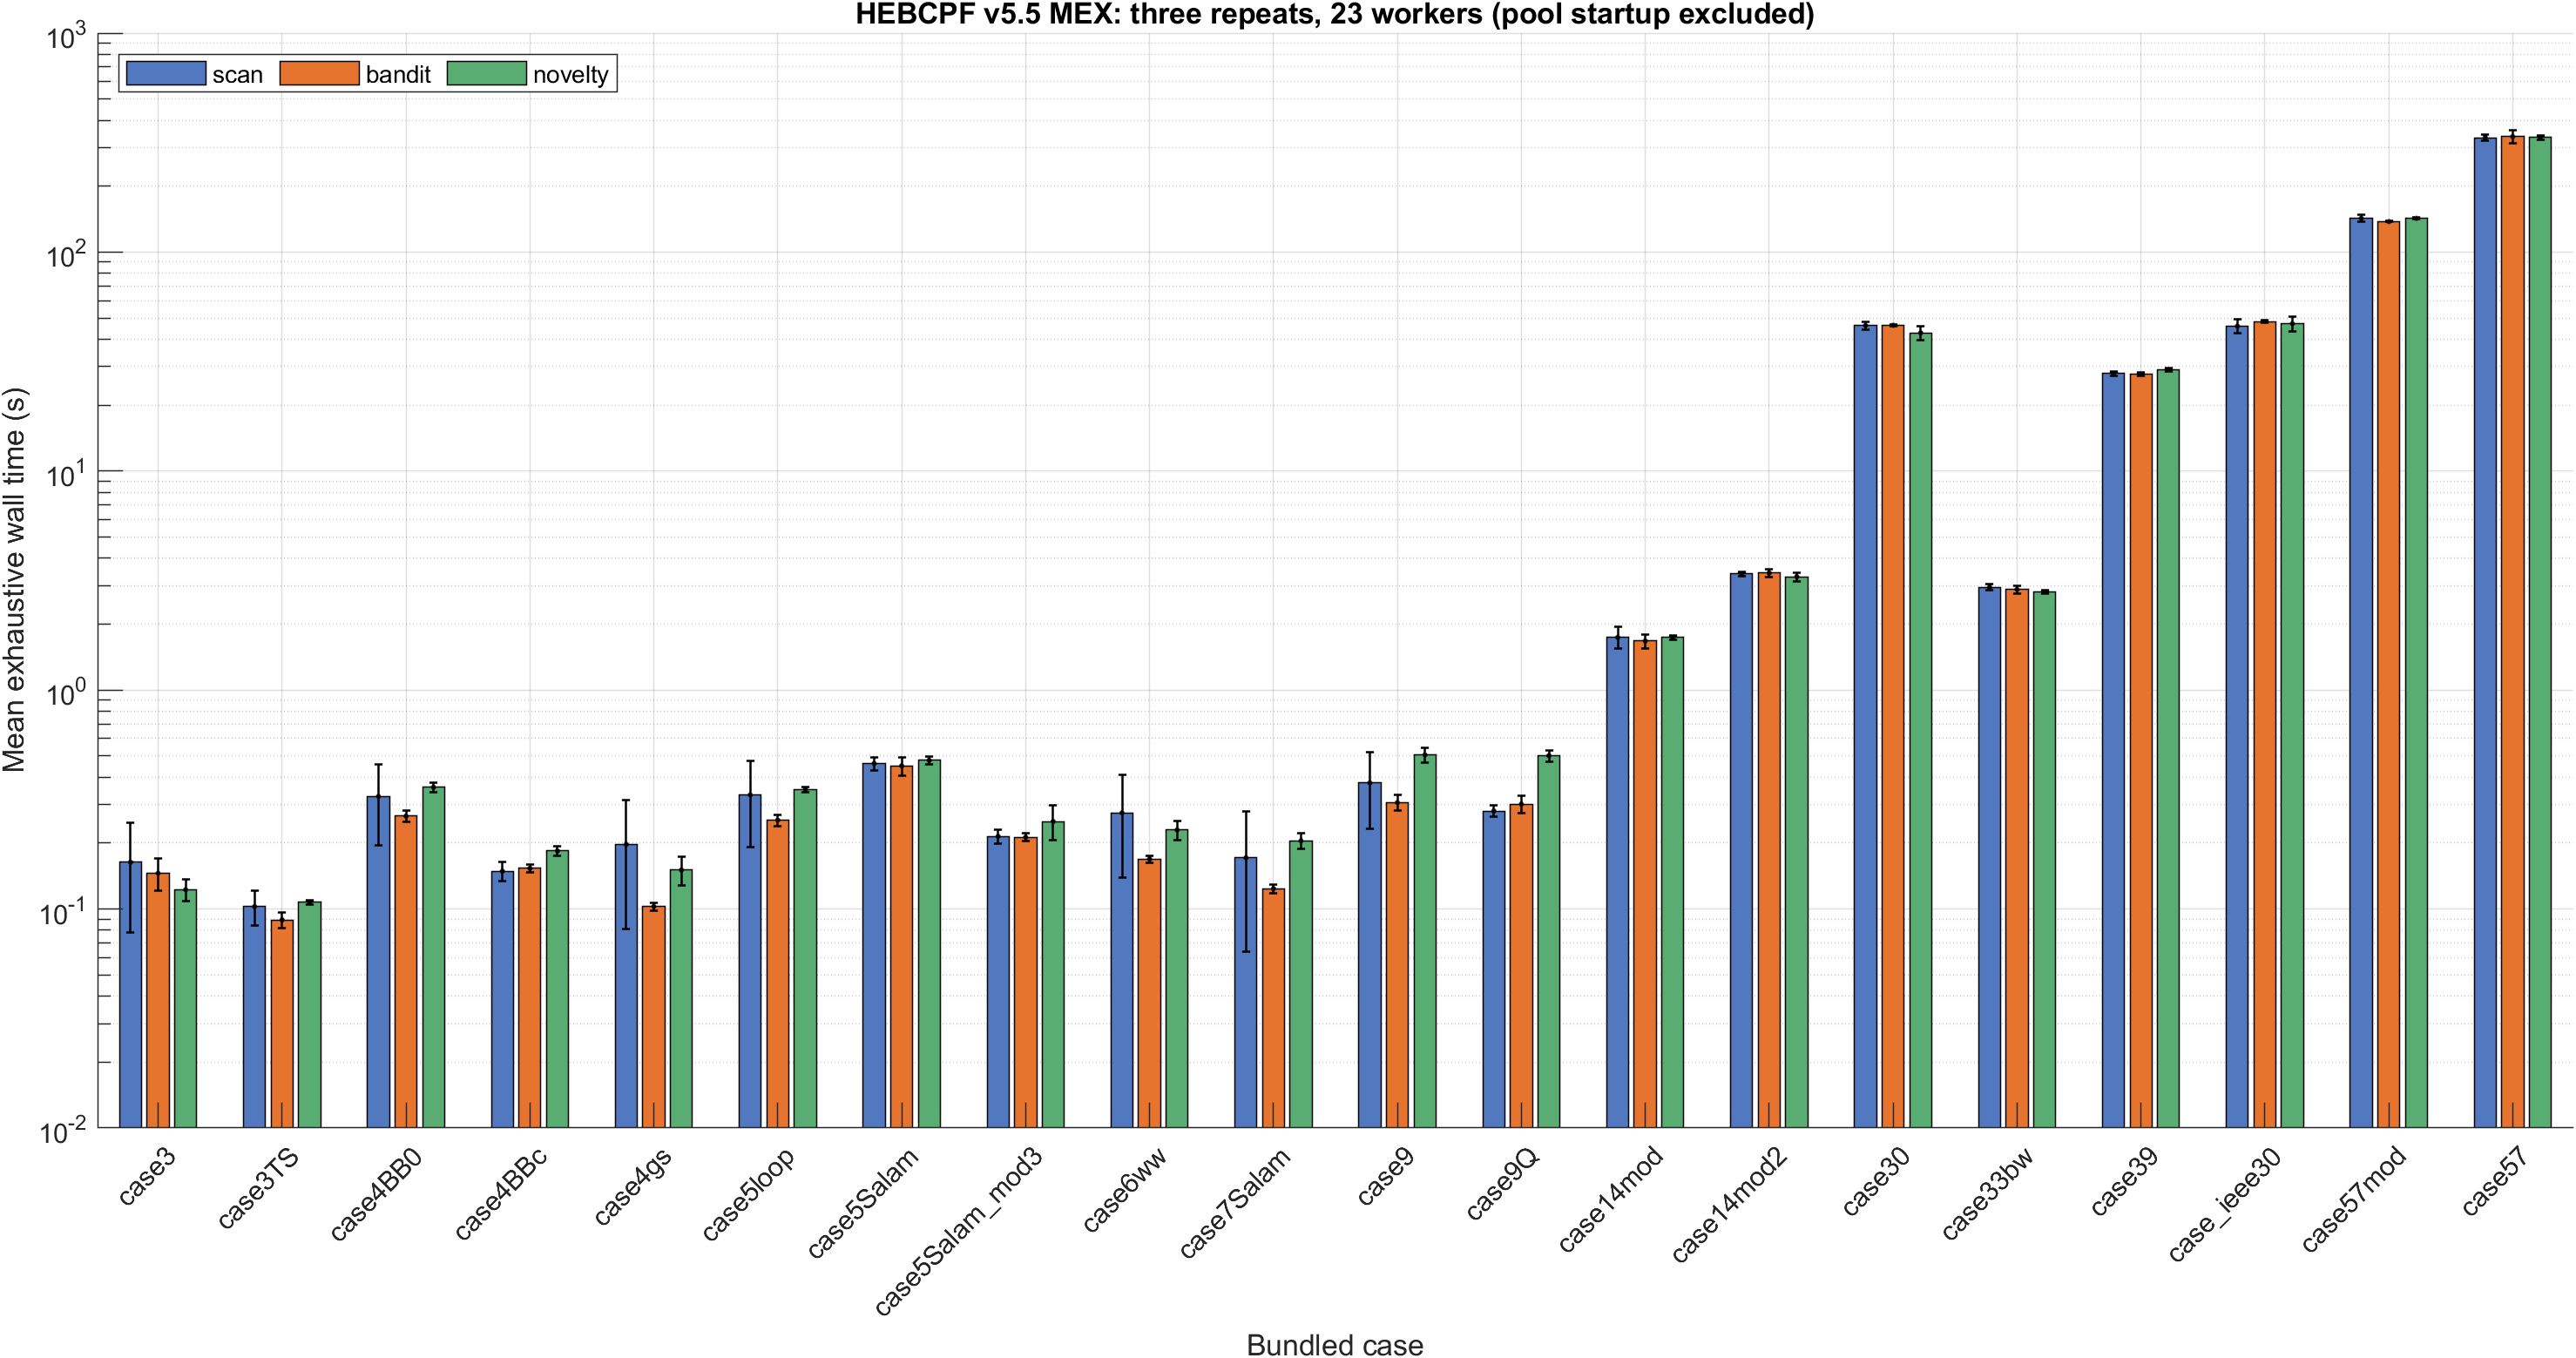
\includegraphics[width=0.96\textwidth]{scheduler_benchmark_v5_wall.png}
\caption{Three-repeat mean exhaustive MEX wall time by scheduler.}
\end{figure}}{}
\IfFileExists{scheduler_benchmark_v5_t90.png}{
\begin{figure}[htbp]\centering
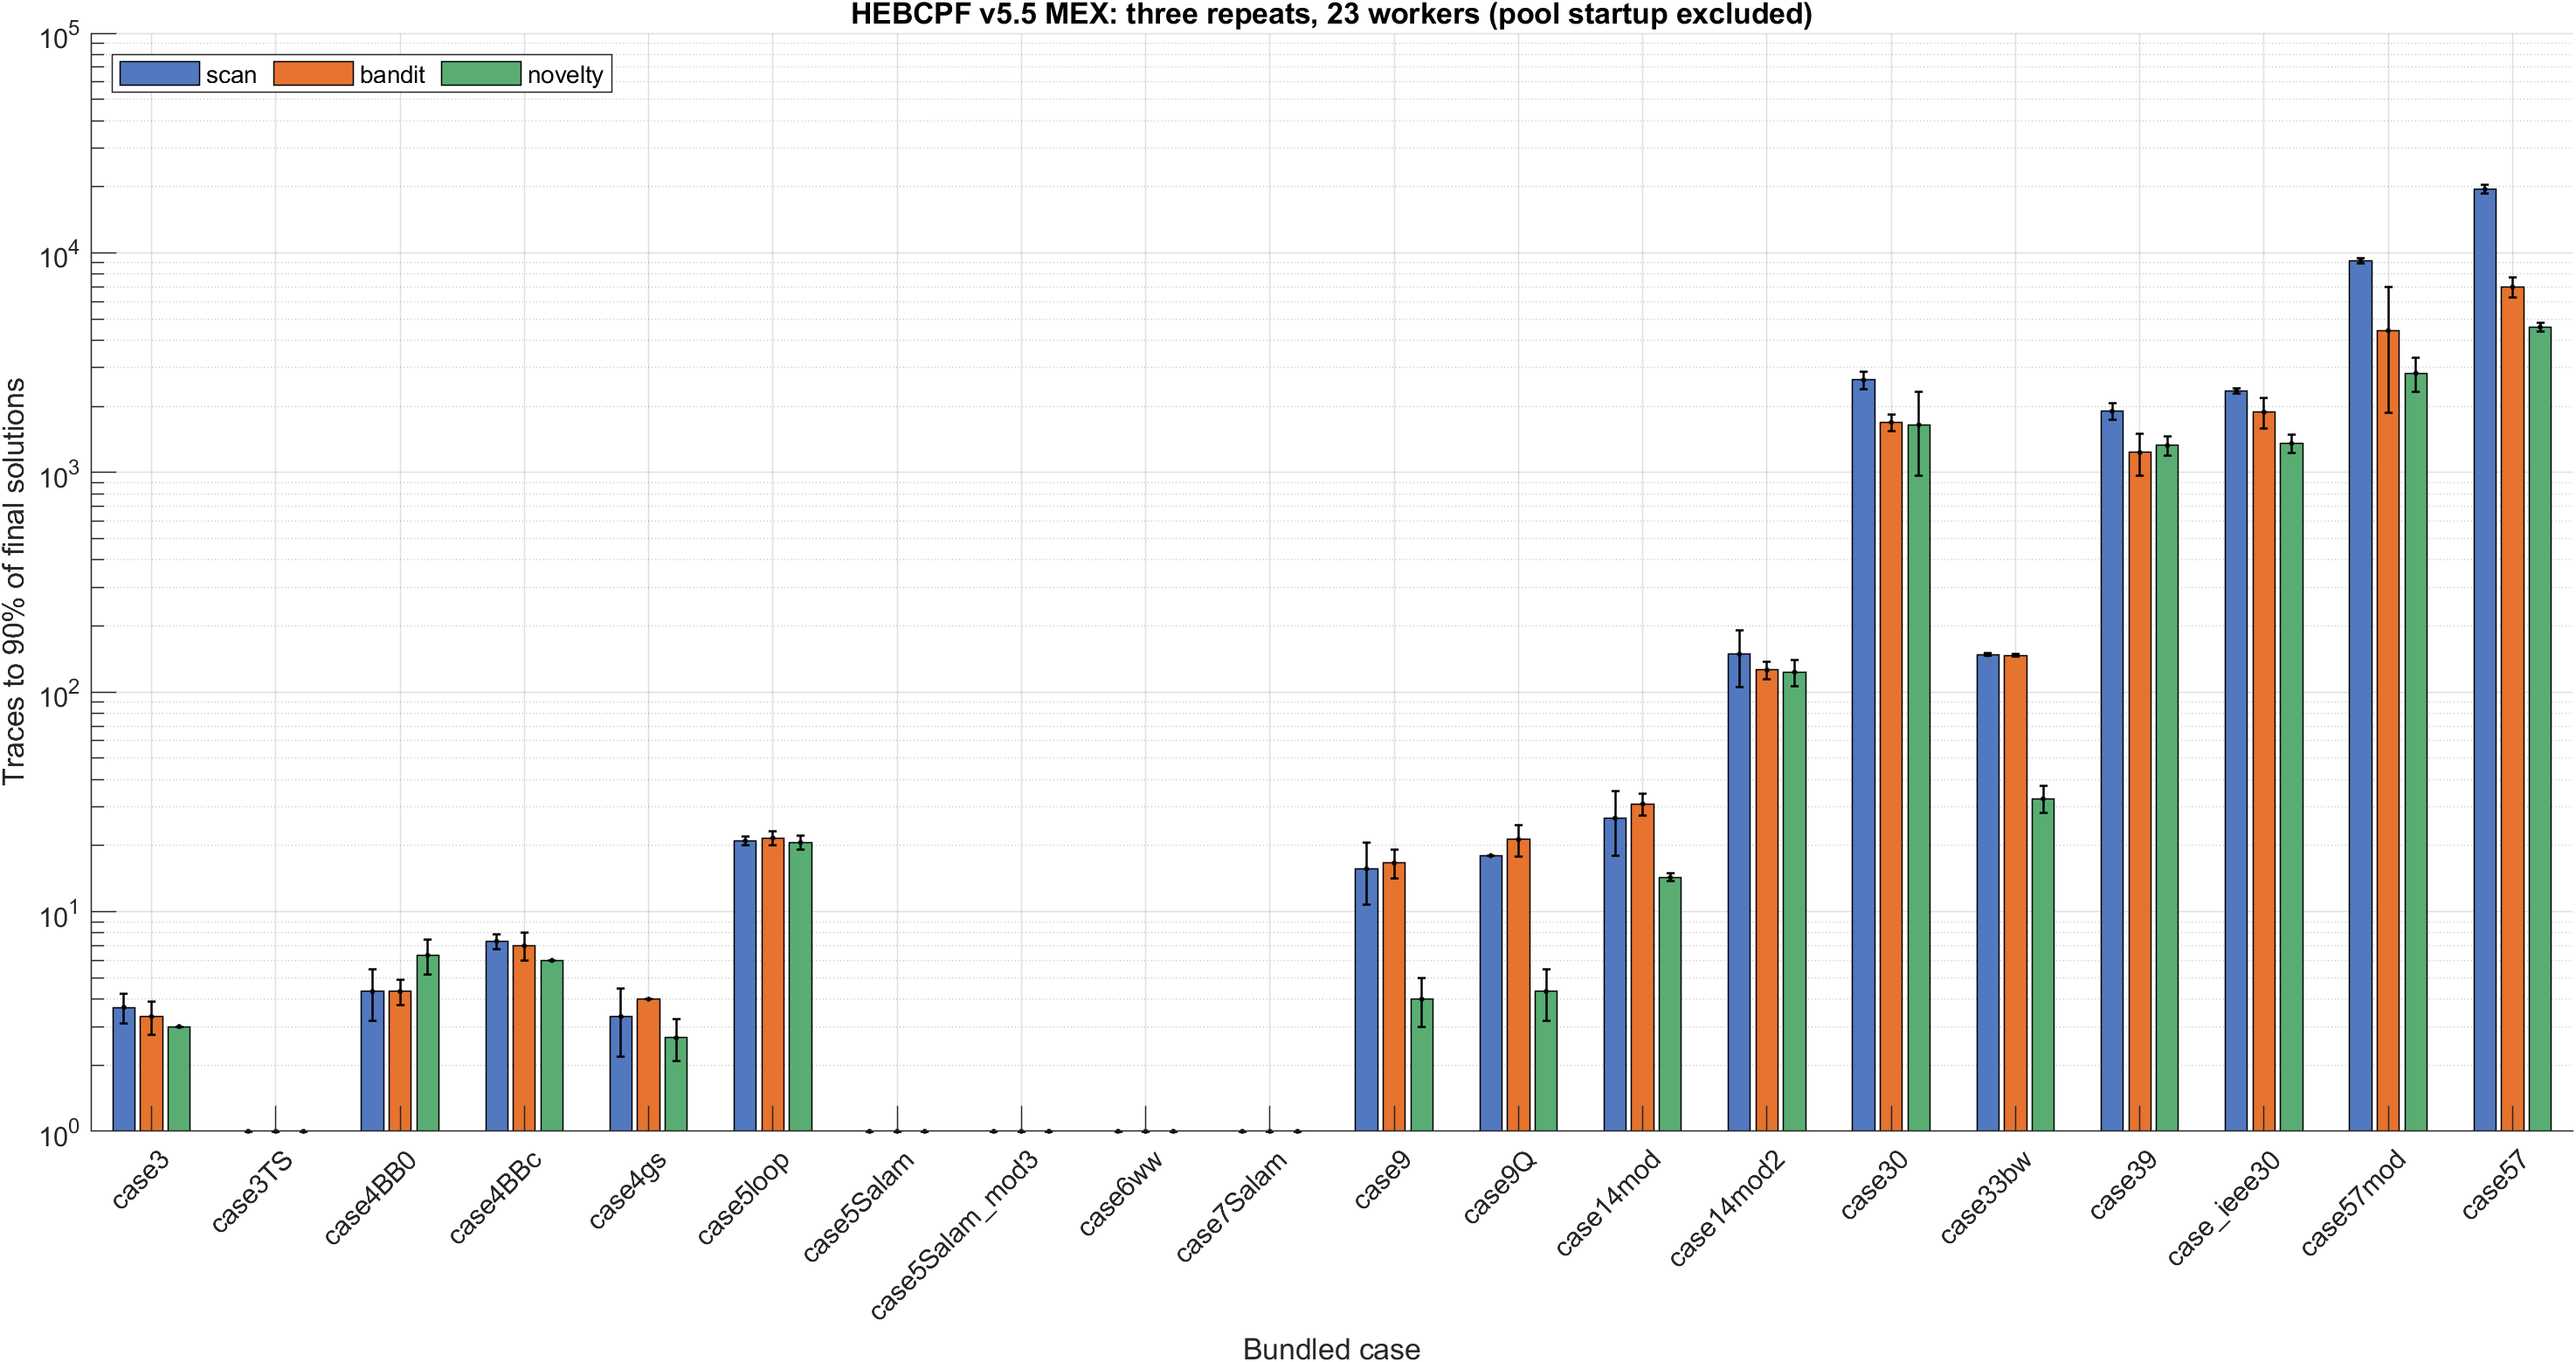
\includegraphics[width=0.96\textwidth]{scheduler_benchmark_v5_t90.png}
\caption{Mean completed traces required to reach 90\% of final solutions.}
\end{figure}}{}
\IfFileExists{scheduler_benchmark_v5_anytime.png}{
\begin{figure}[htbp]\centering
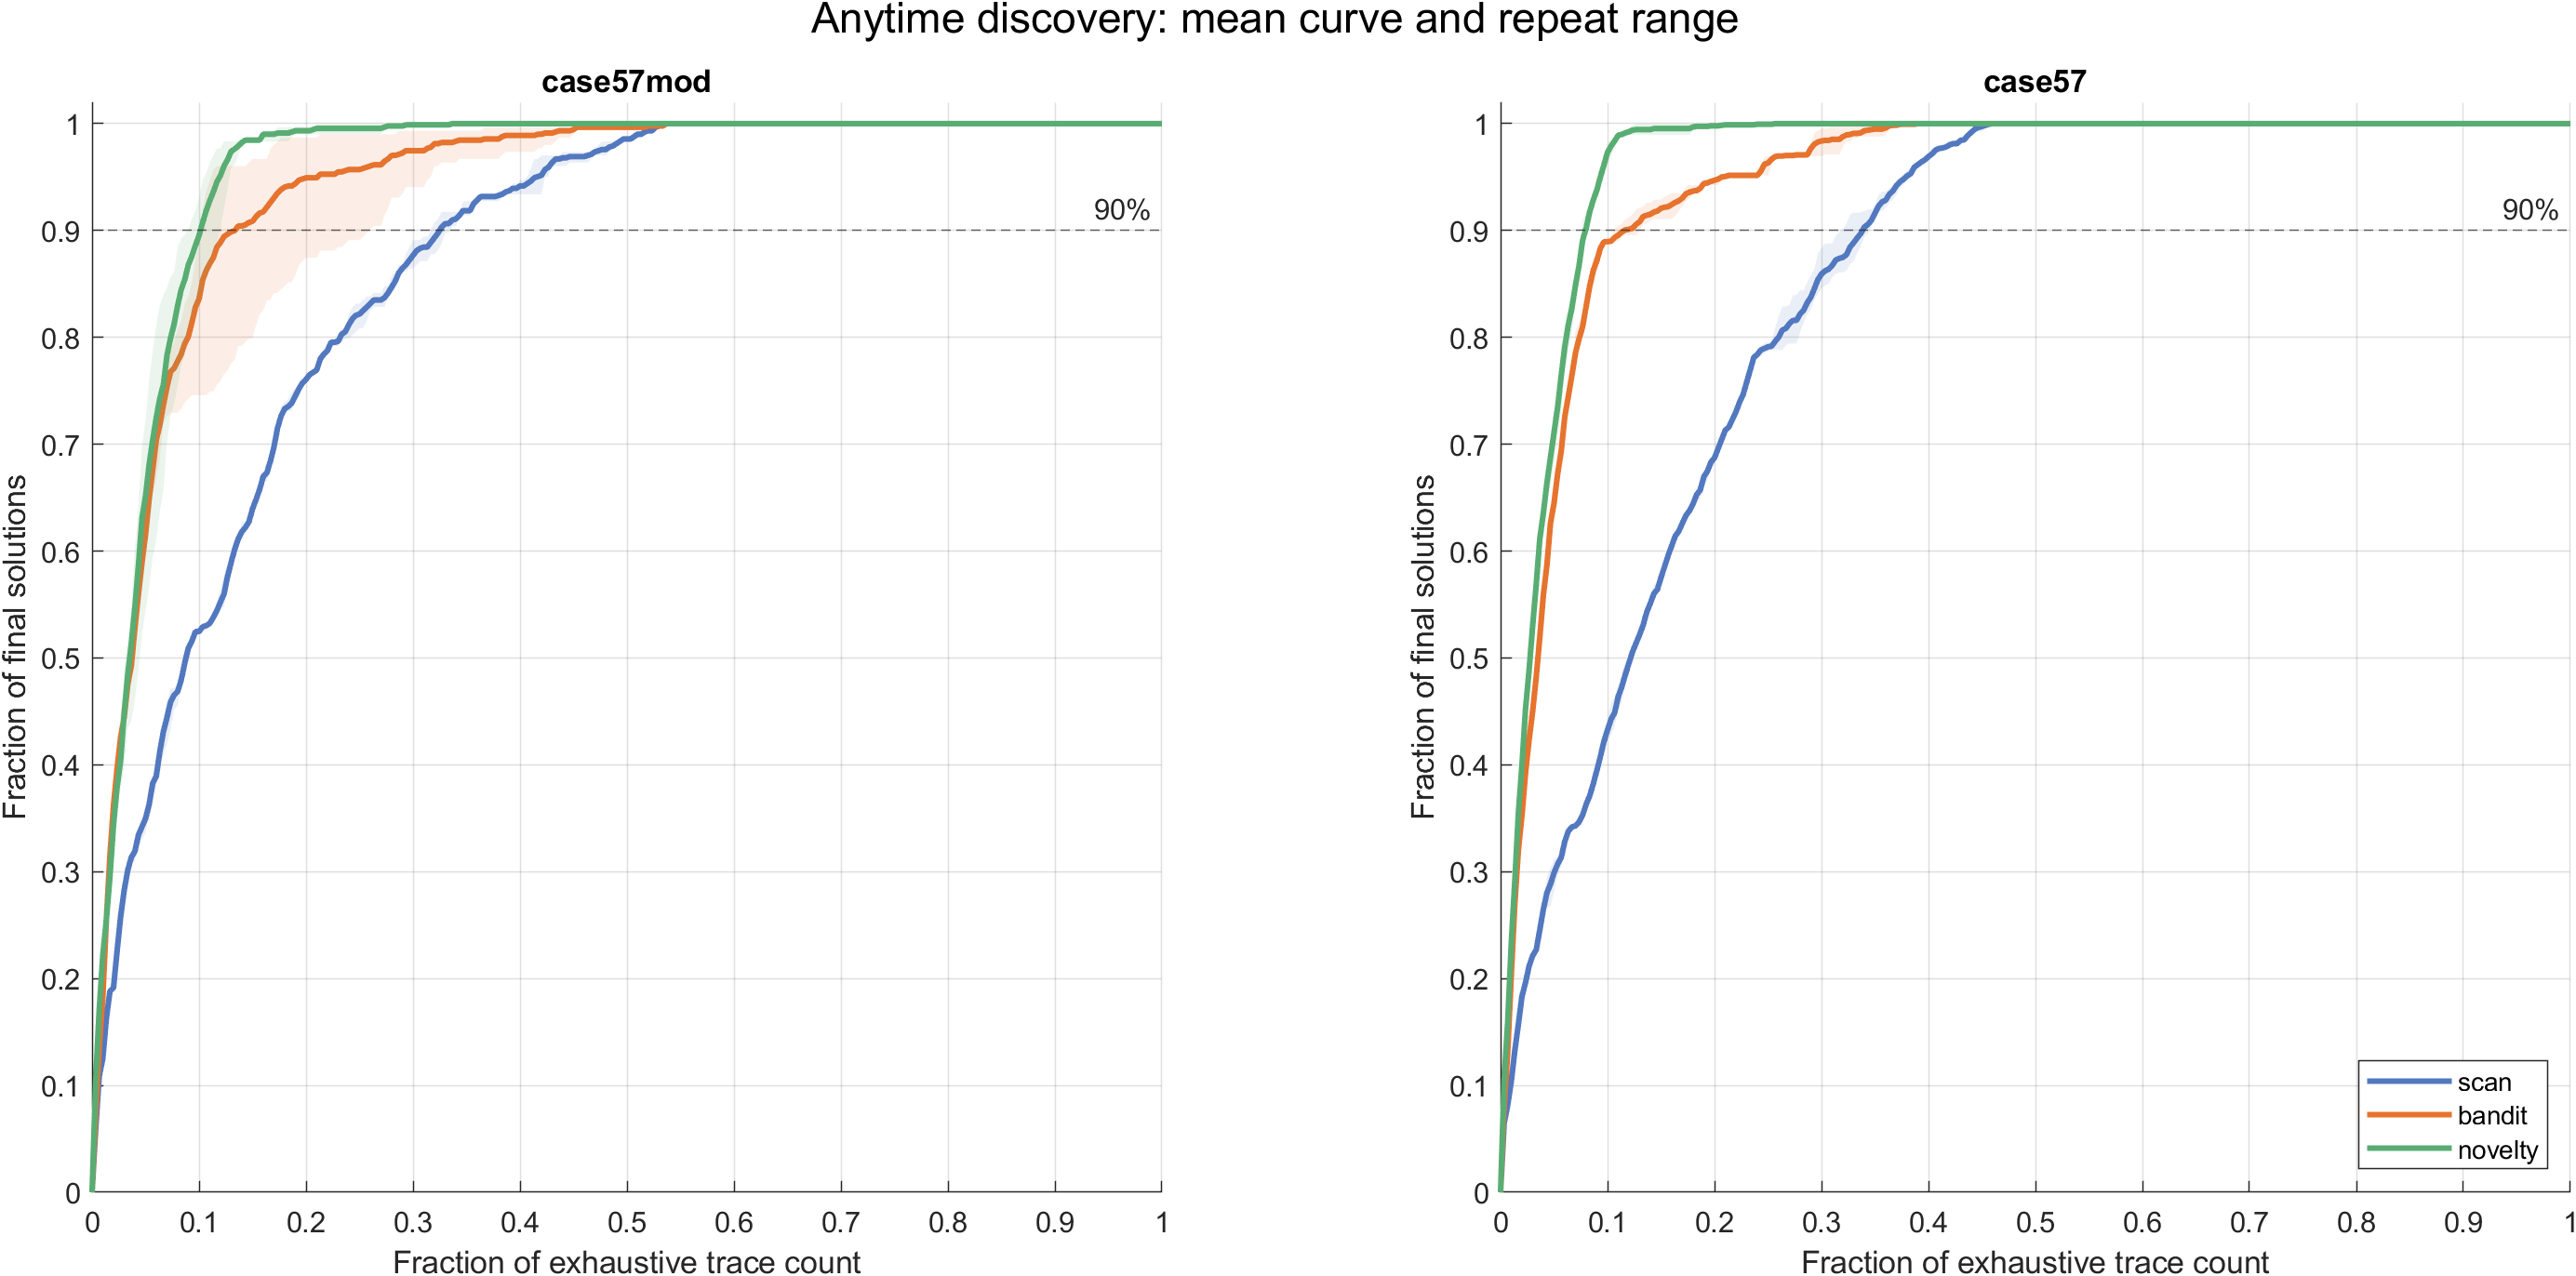
\includegraphics[width=0.96\textwidth]{scheduler_benchmark_v5_anytime.png}
\caption{Anytime discovery for case57mod and case57; bands span three repeats.}
\end{figure}}{}
\IfFileExists{scheduler_benchmark_v5_anytime_representative.png}{
\begin{figure}[htbp]\centering
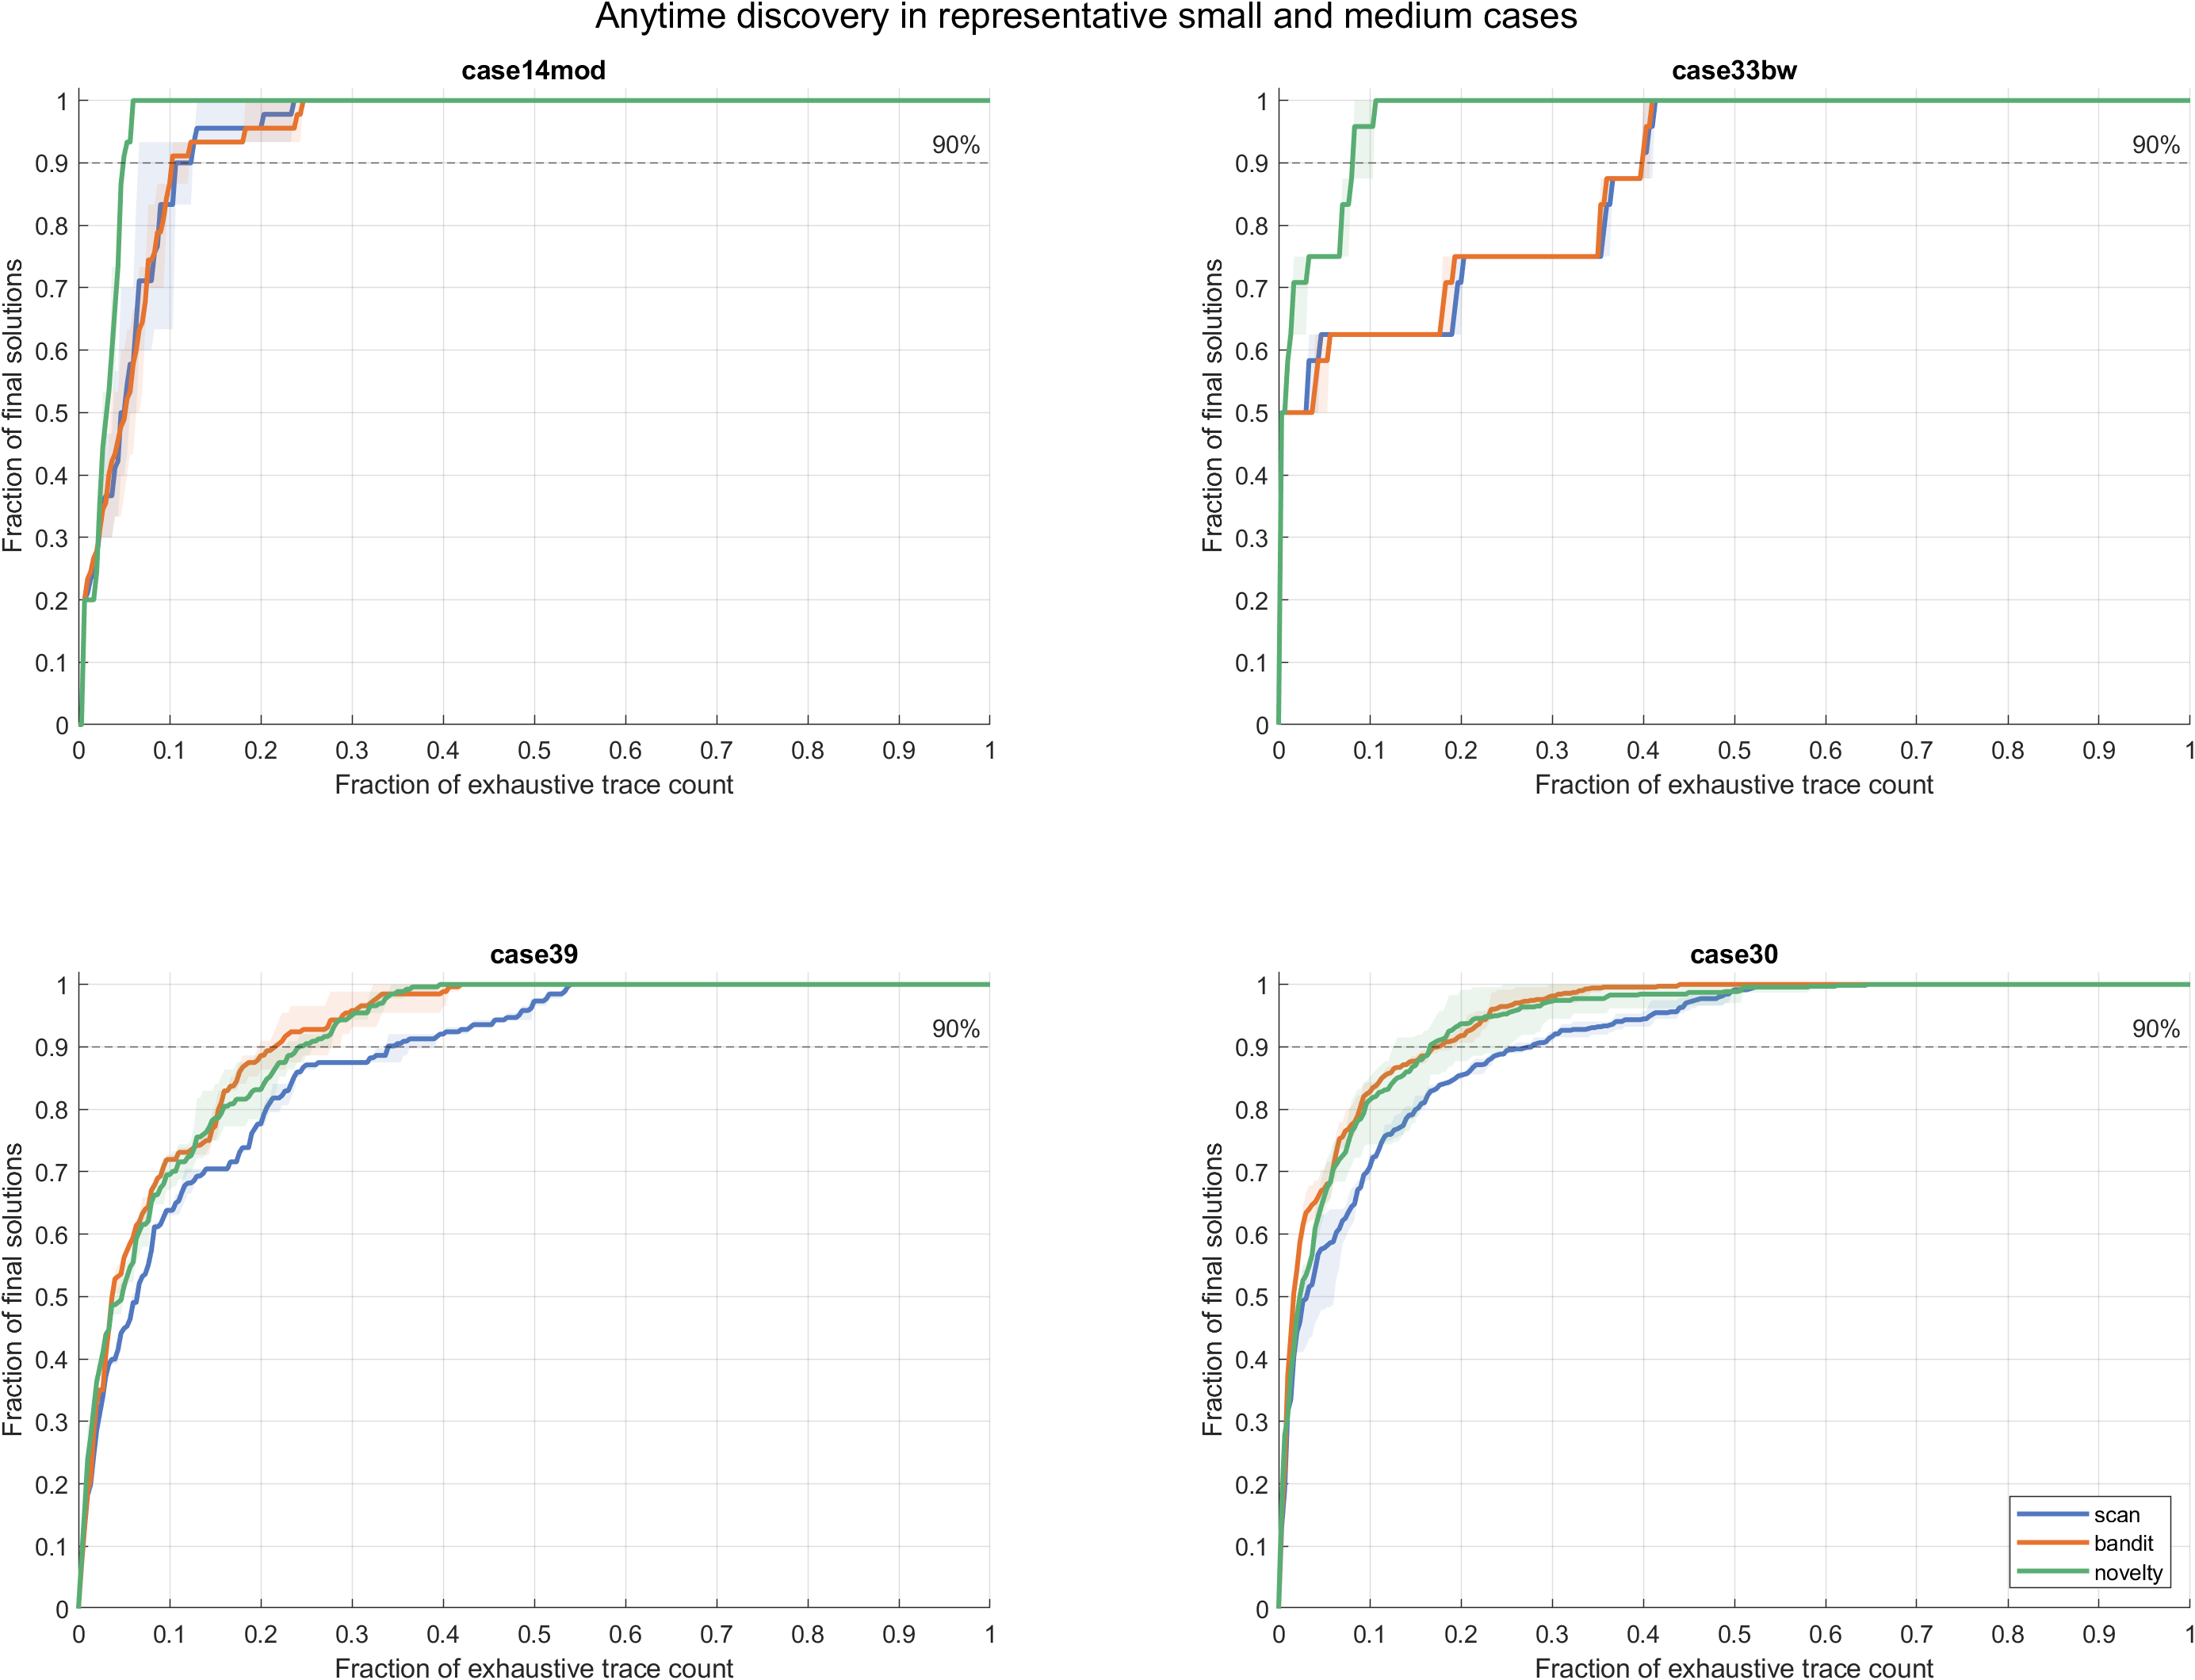
\includegraphics[width=0.96\textwidth]{scheduler_benchmark_v5_anytime_representative.png}
\caption{Recorded anytime discovery for case14mod, case33bw, case39, and case30.
Each line is the three-repeat mean and each band spans the repeat range. These
additional panels are reconstructed from saved trace histories; no solver was rerun.}
\end{figure}}{}
\IfFileExists{scheduler_benchmark_v5_anytime_suite.png}{
\begin{figure}[htbp]\centering
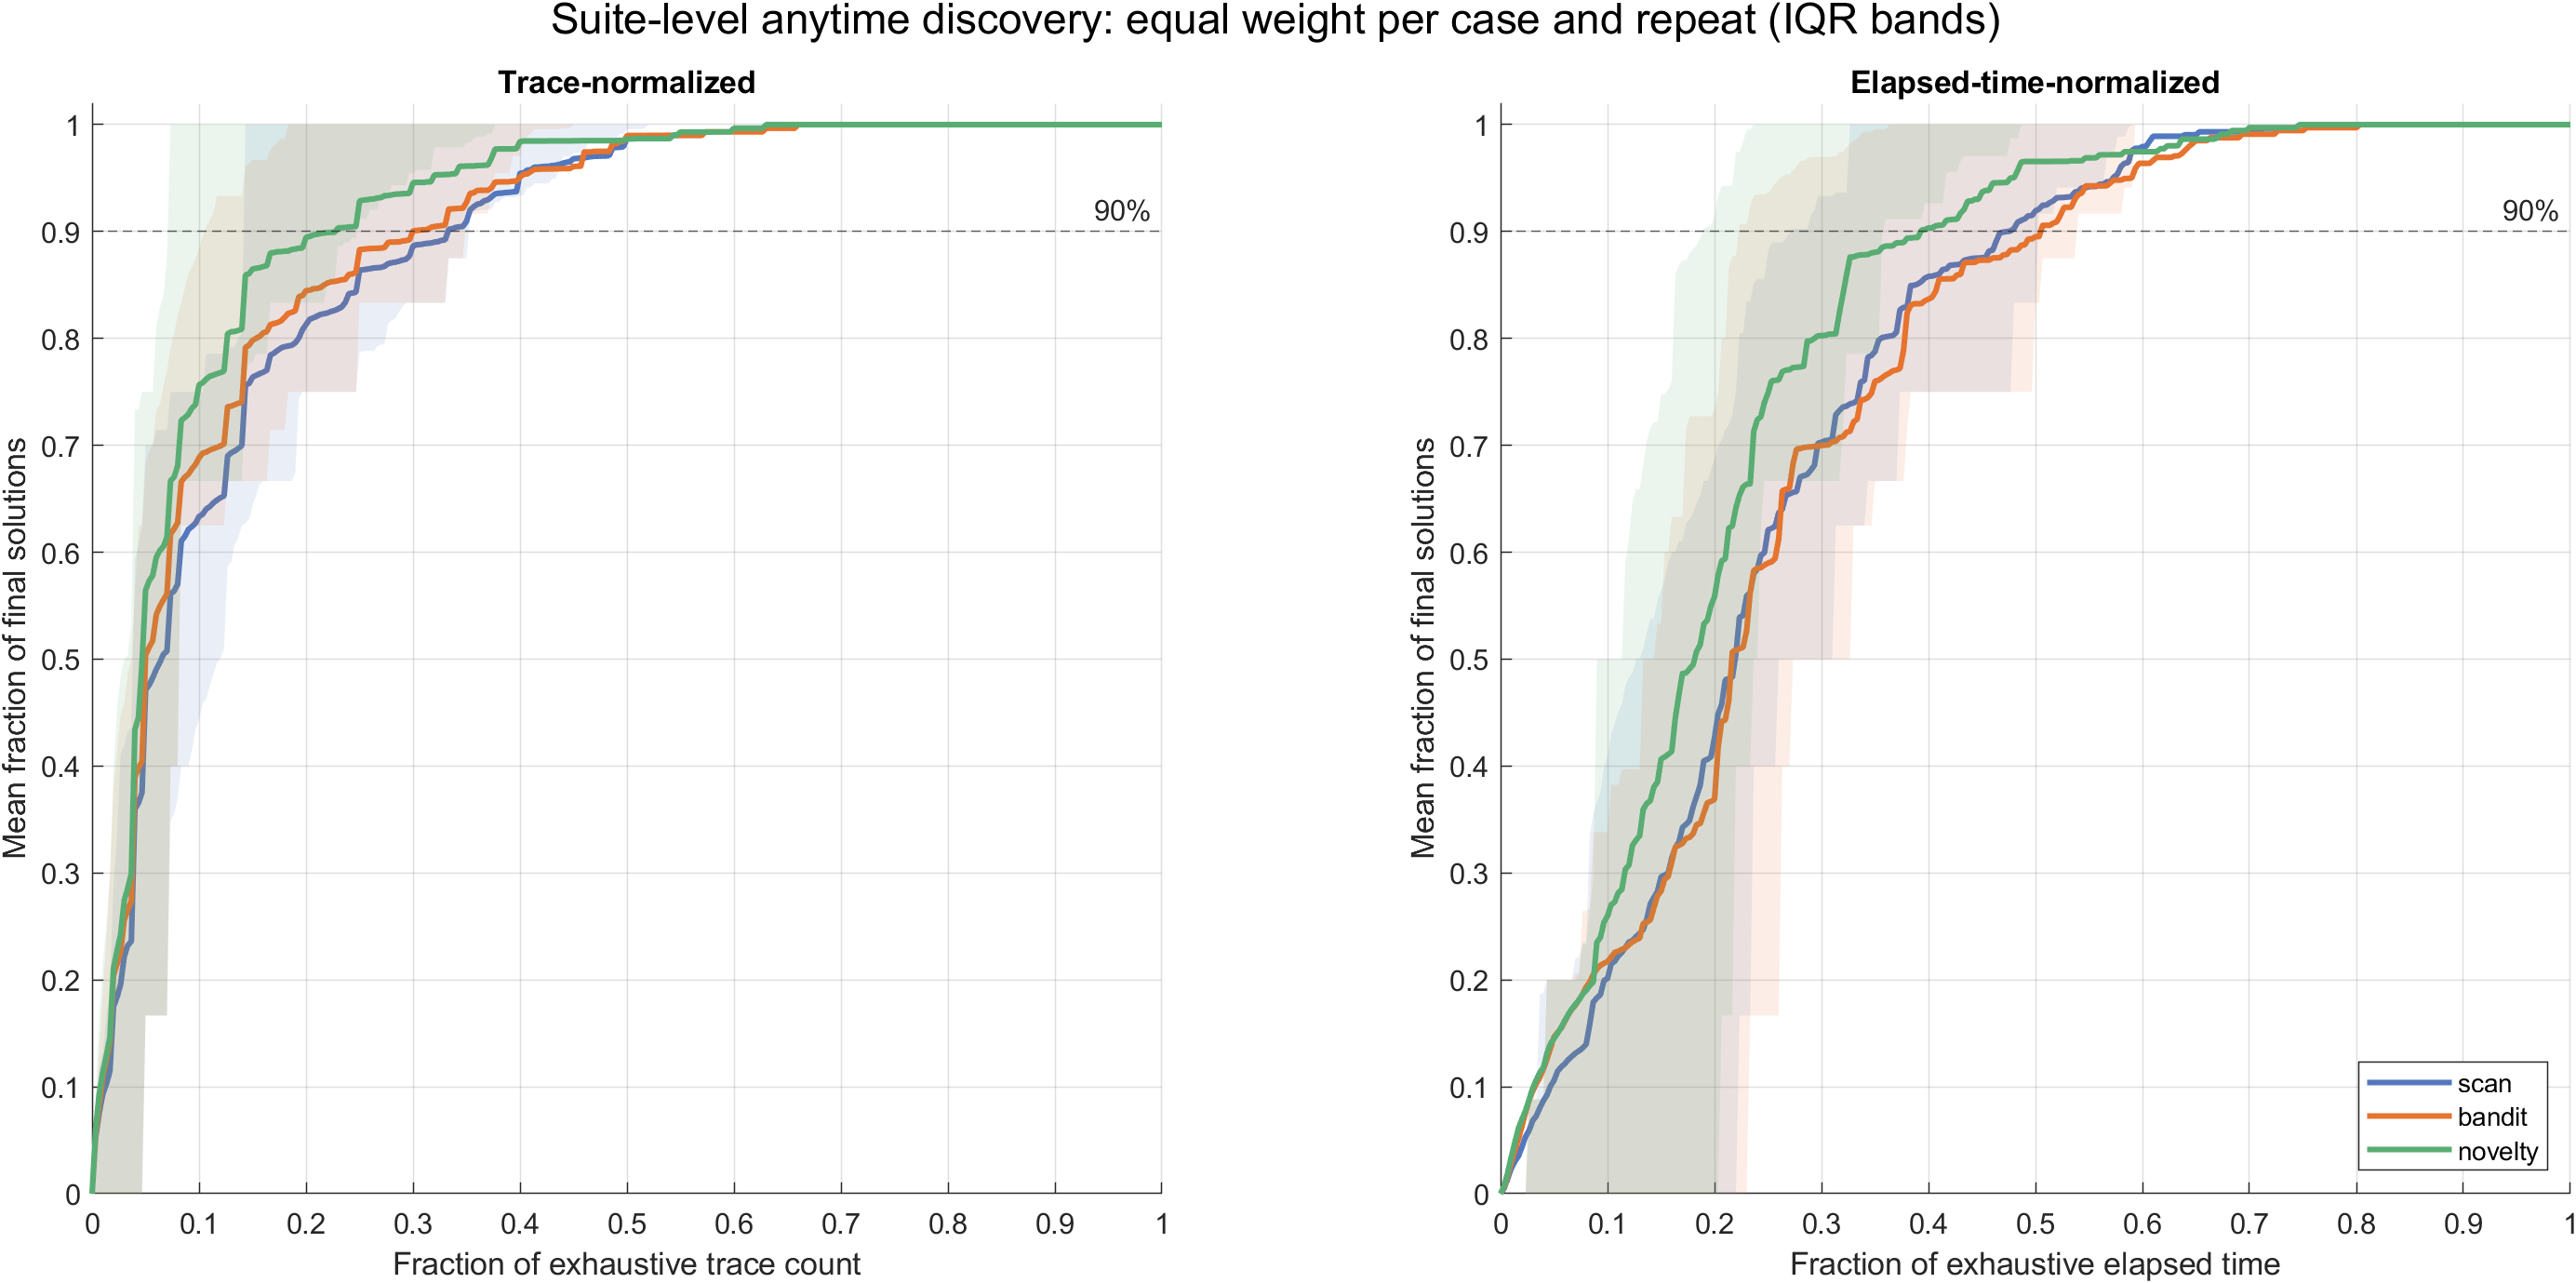
\includegraphics[width=0.96\textwidth]{scheduler_benchmark_v5_anytime_suite.png}
\caption{Suite-level normalized anytime discovery over all 20 cases. Every case
and repeat receives equal weight; bands show the interquartile range. The left
panel normalizes by exhaustive traces and the right by exhaustive elapsed time.}
\end{figure}}{}

The added case panels show that adaptive ordering is not only a case57 effect,
although the size of the advantage varies with topology and solution count. The
suite-level macro average deliberately weights every case equally, so it describes
typical normalized progress rather than allowing the two case57 variants to dominate.

The connectivity panels use one common layout per case. Nodes are accepted
solutions, color is discovery order, and edges link solutions covered by a
shared trace. Differences describe traversal history, not different final sets.

\IfFileExists{connectivity_case14mod_scan.png}{
\begin{figure}[htbp]\centering
\begin{tabular}{ccc}
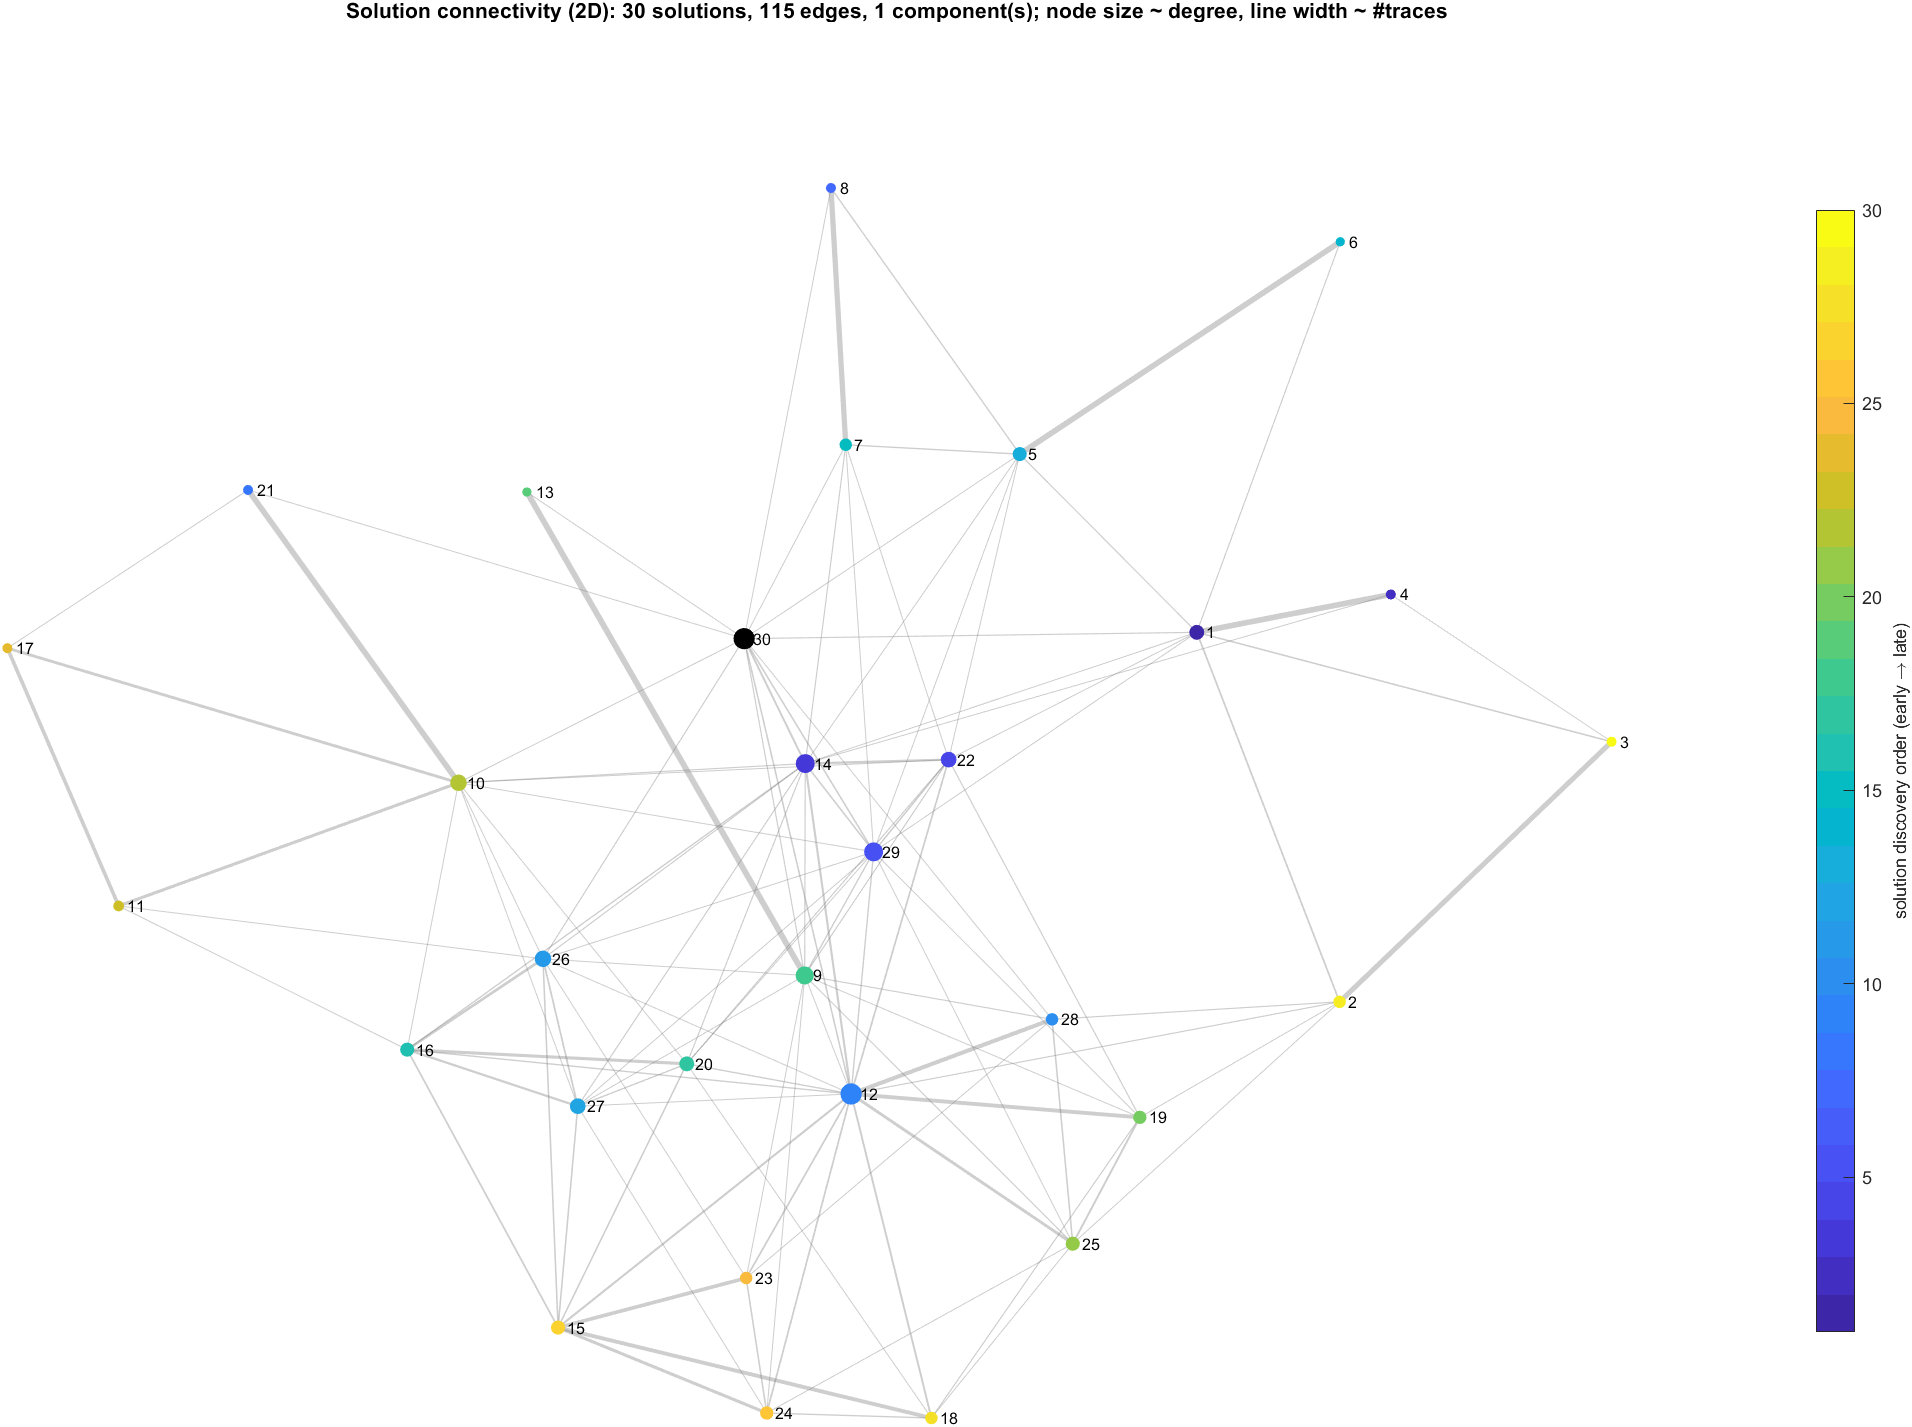
\includegraphics[width=0.30\textwidth]{connectivity_case14mod_scan.png}&
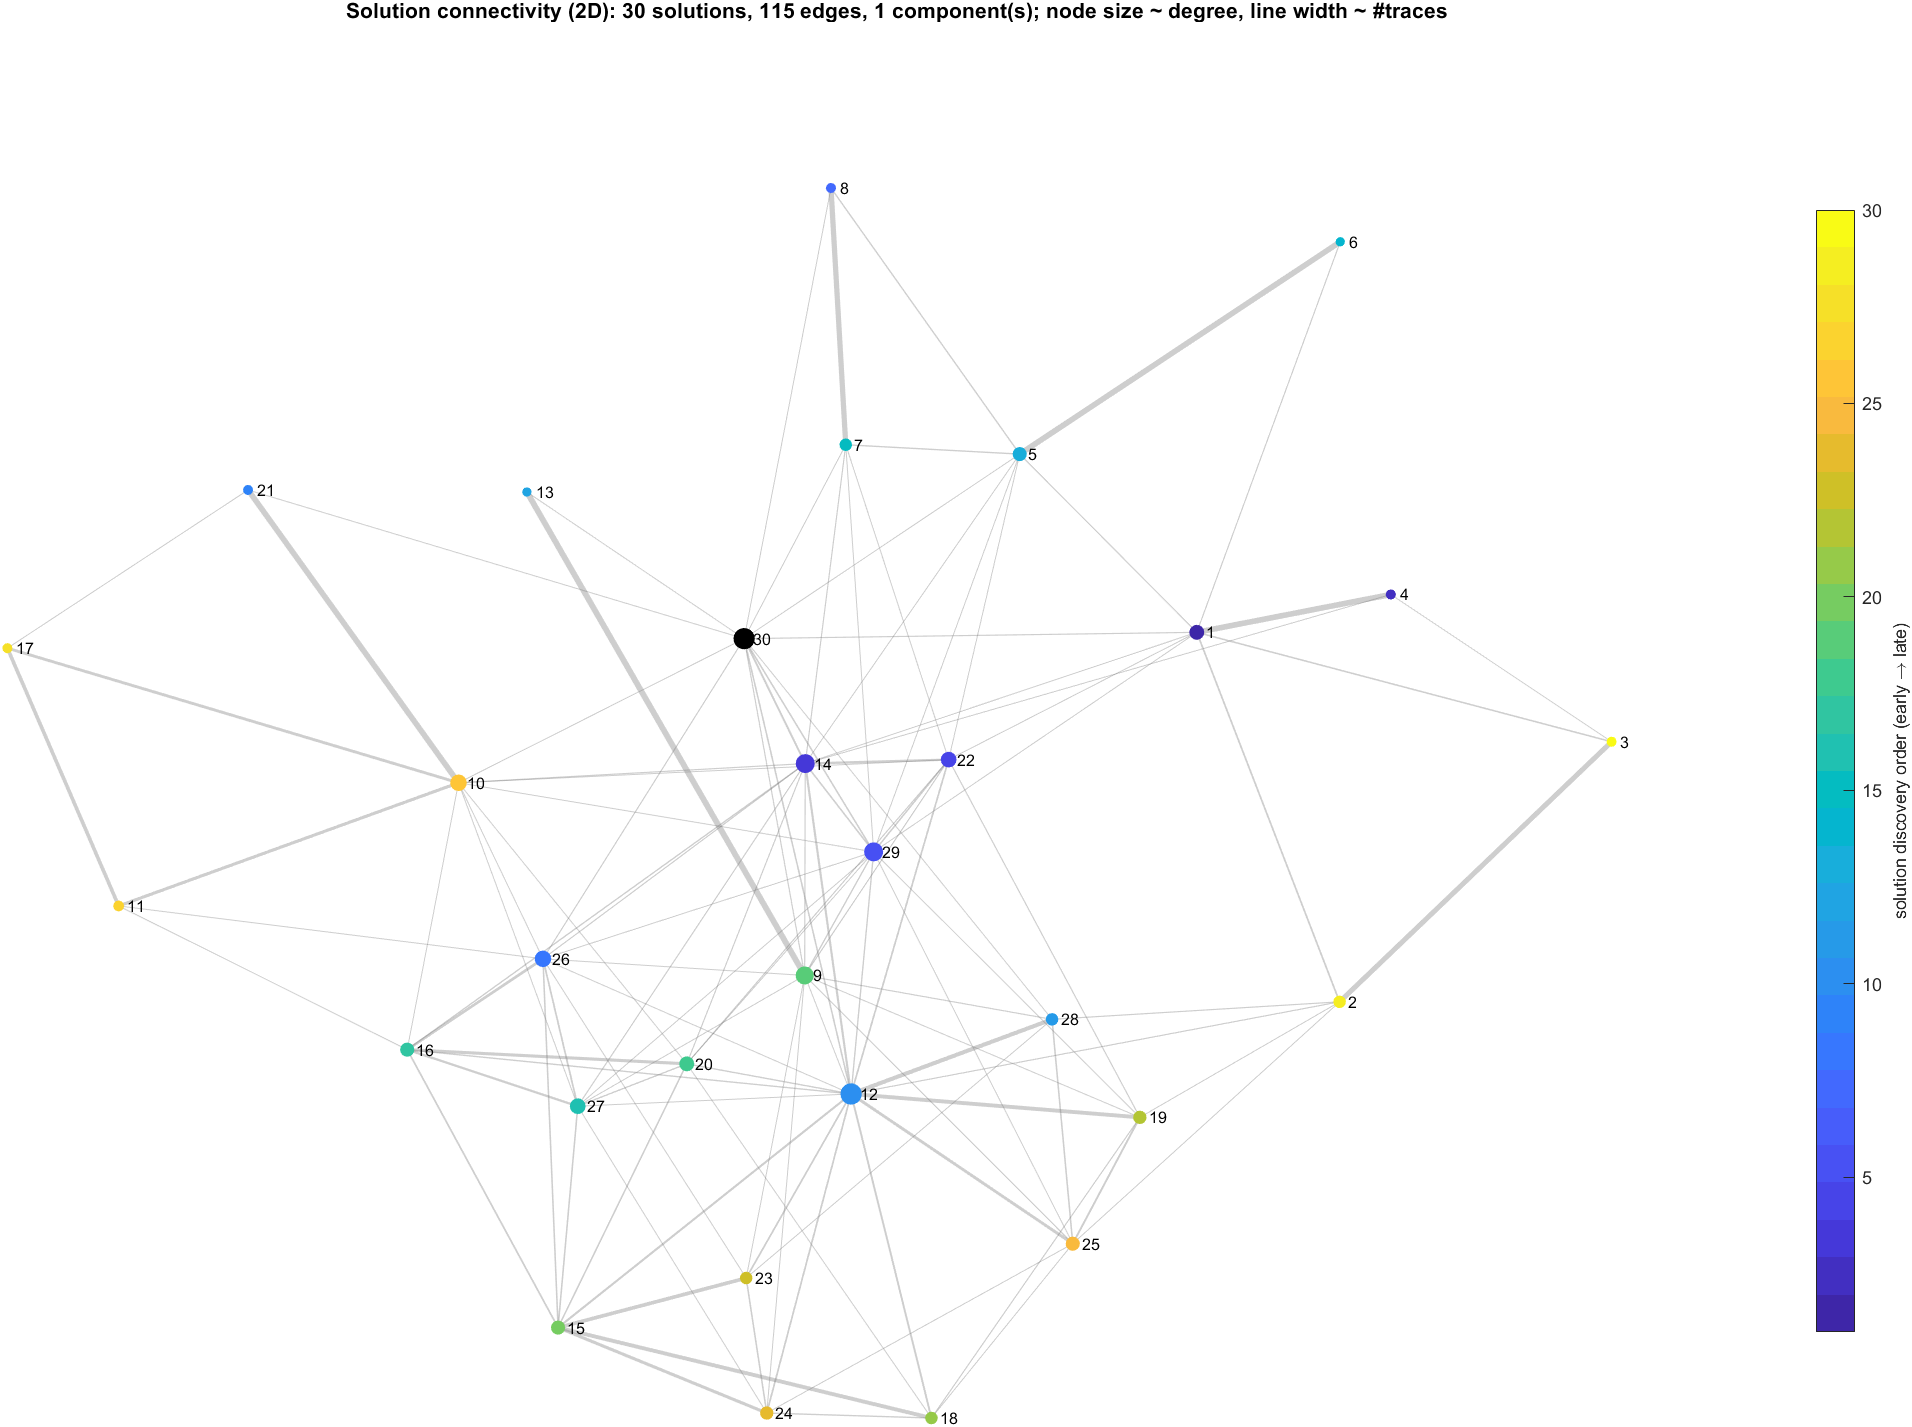
\includegraphics[width=0.30\textwidth]{connectivity_case14mod_bandit.png}&
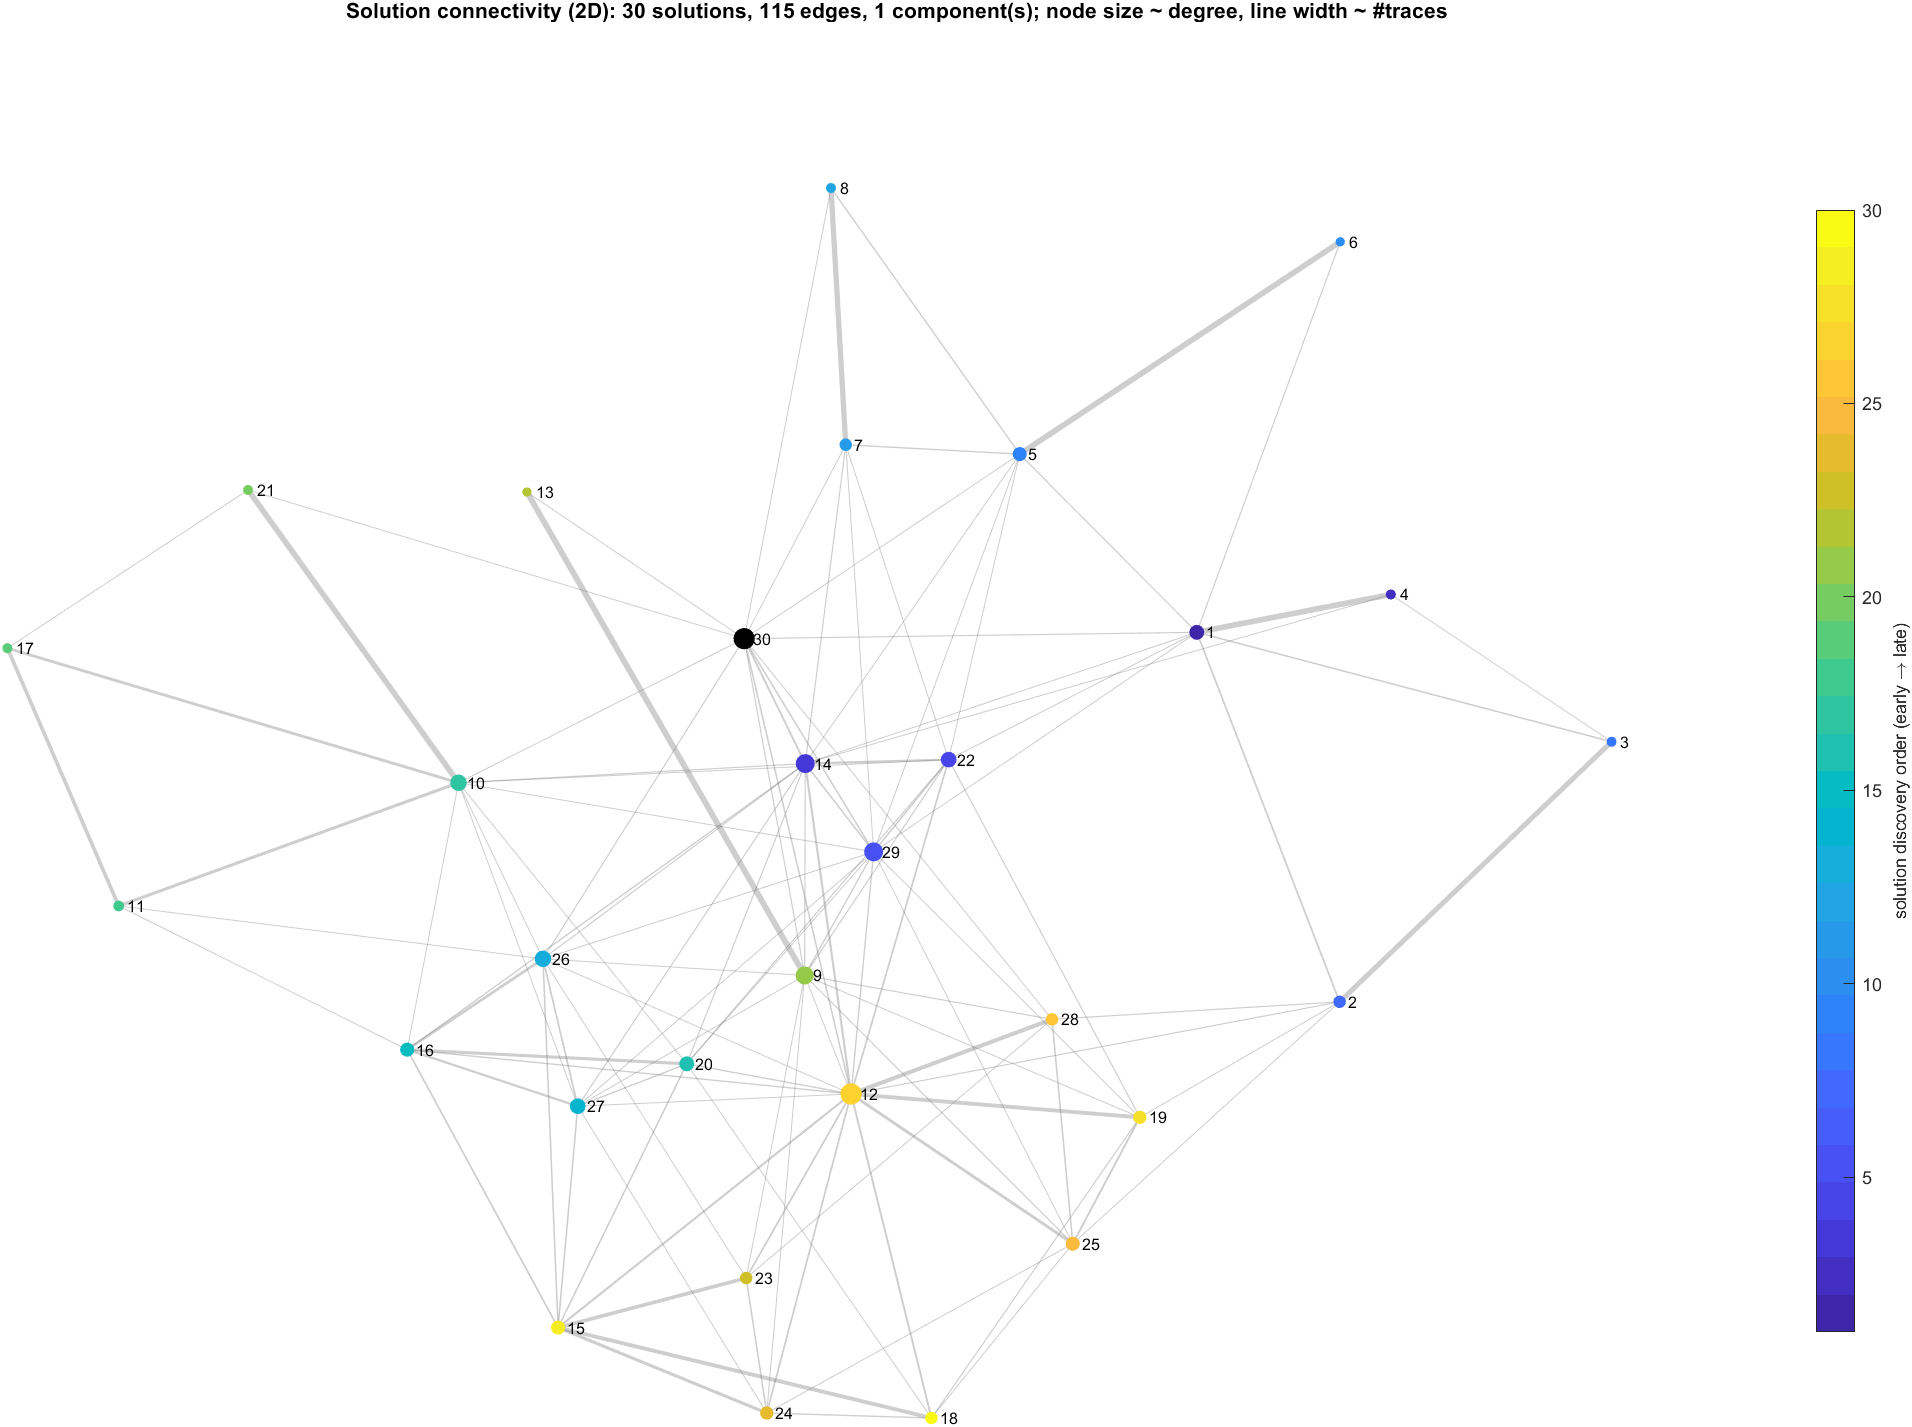
\includegraphics[width=0.30\textwidth]{connectivity_case14mod_novelty.png}\\
\code{scan}&\code{bandit}&\code{novelty}
\end{tabular}
\caption{case14mod connectivity for the common 30-solution set.}
\end{figure}}{}
\IfFileExists{connectivity_case39_scan.png}{
\begin{figure}[htbp]\centering
\begin{tabular}{ccc}
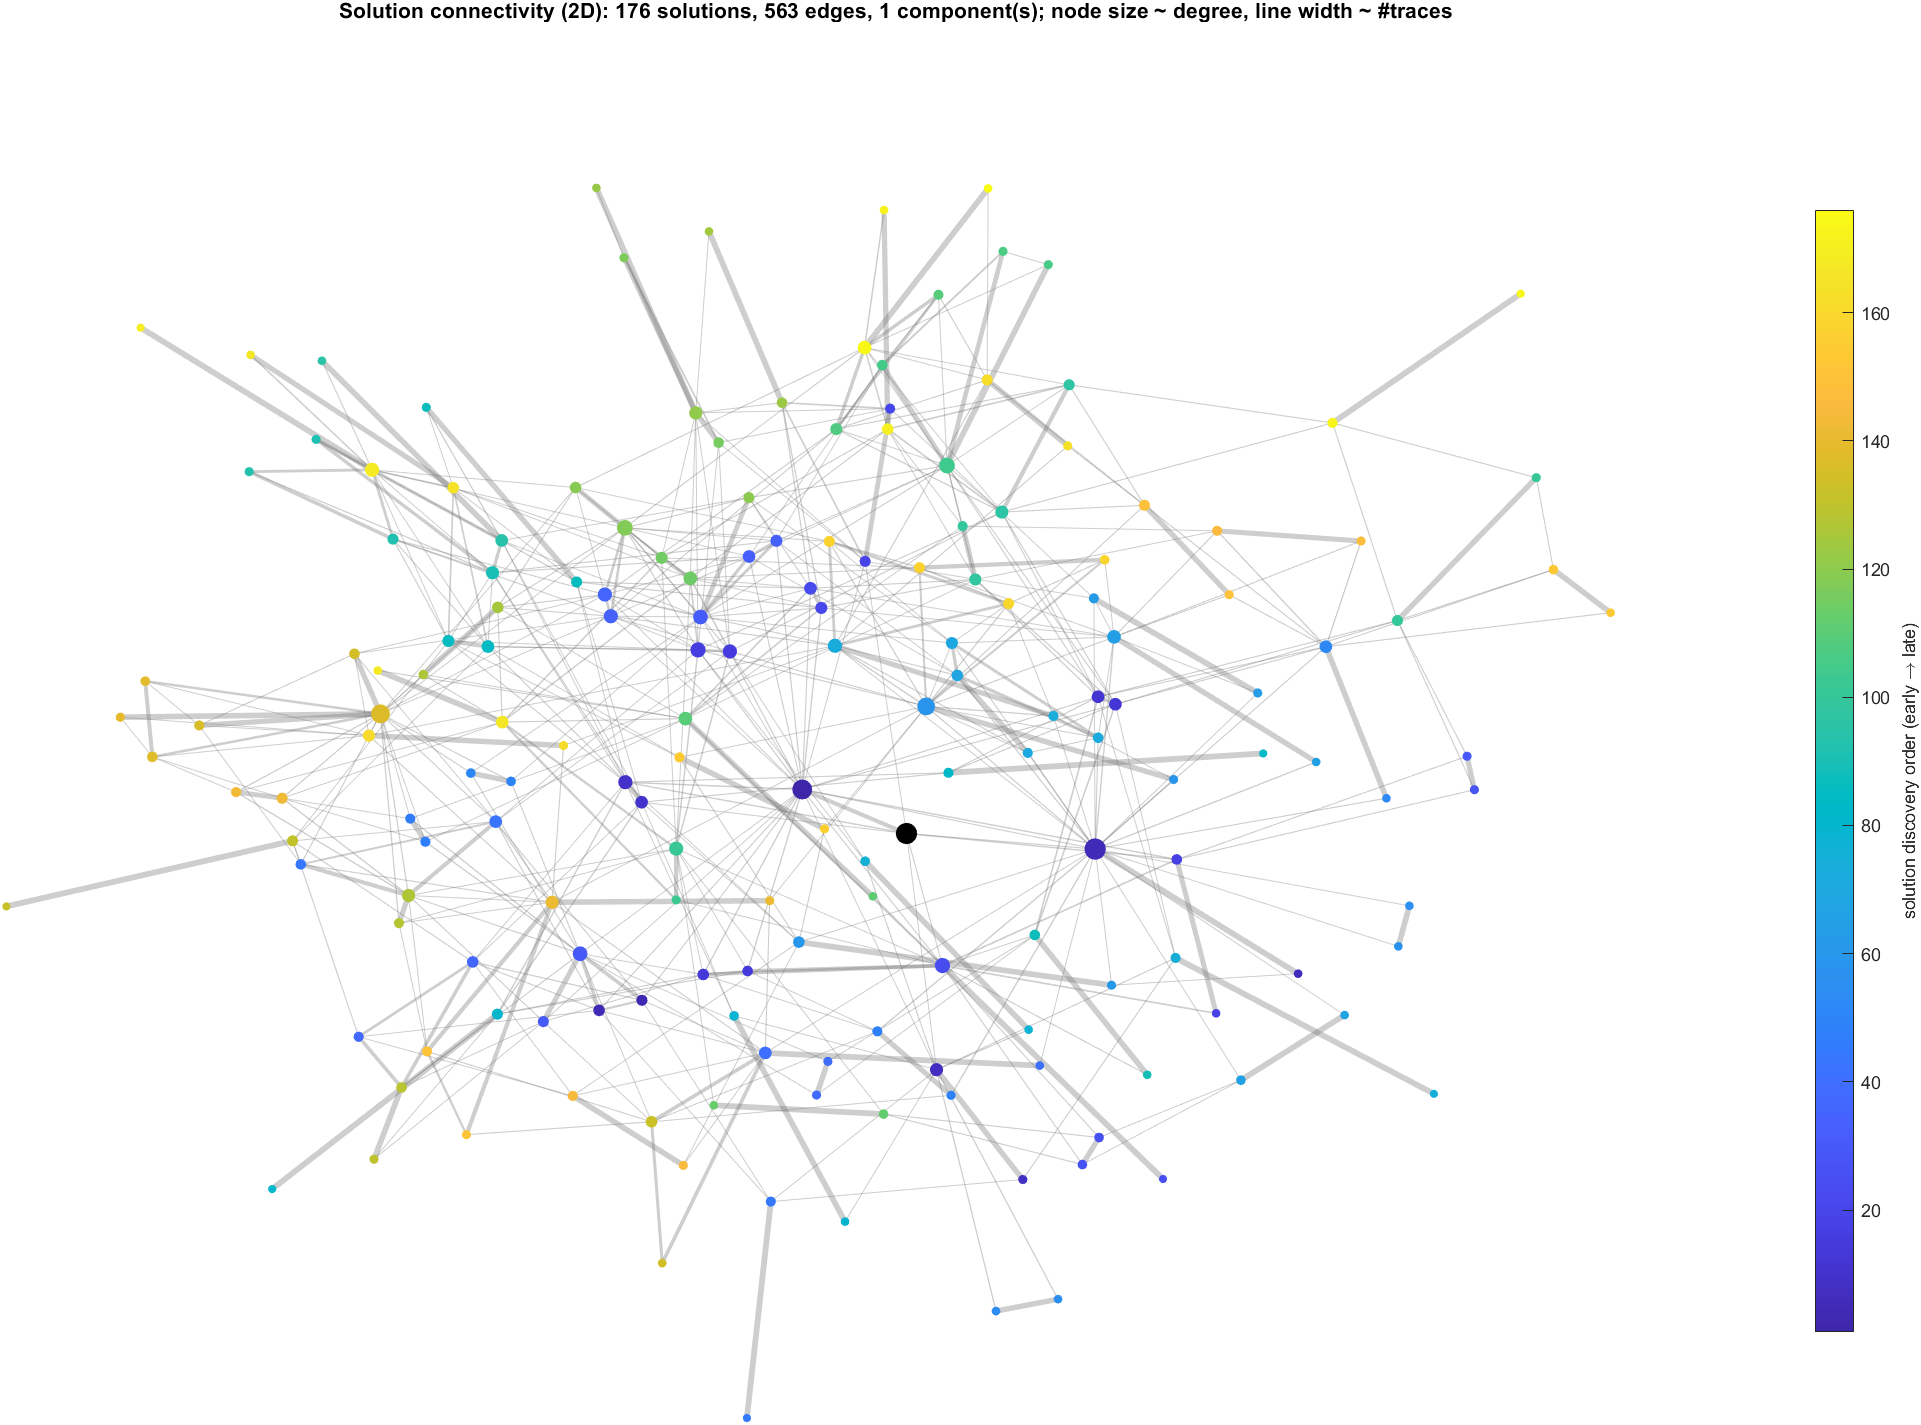
\includegraphics[width=0.30\textwidth]{connectivity_case39_scan.png}&
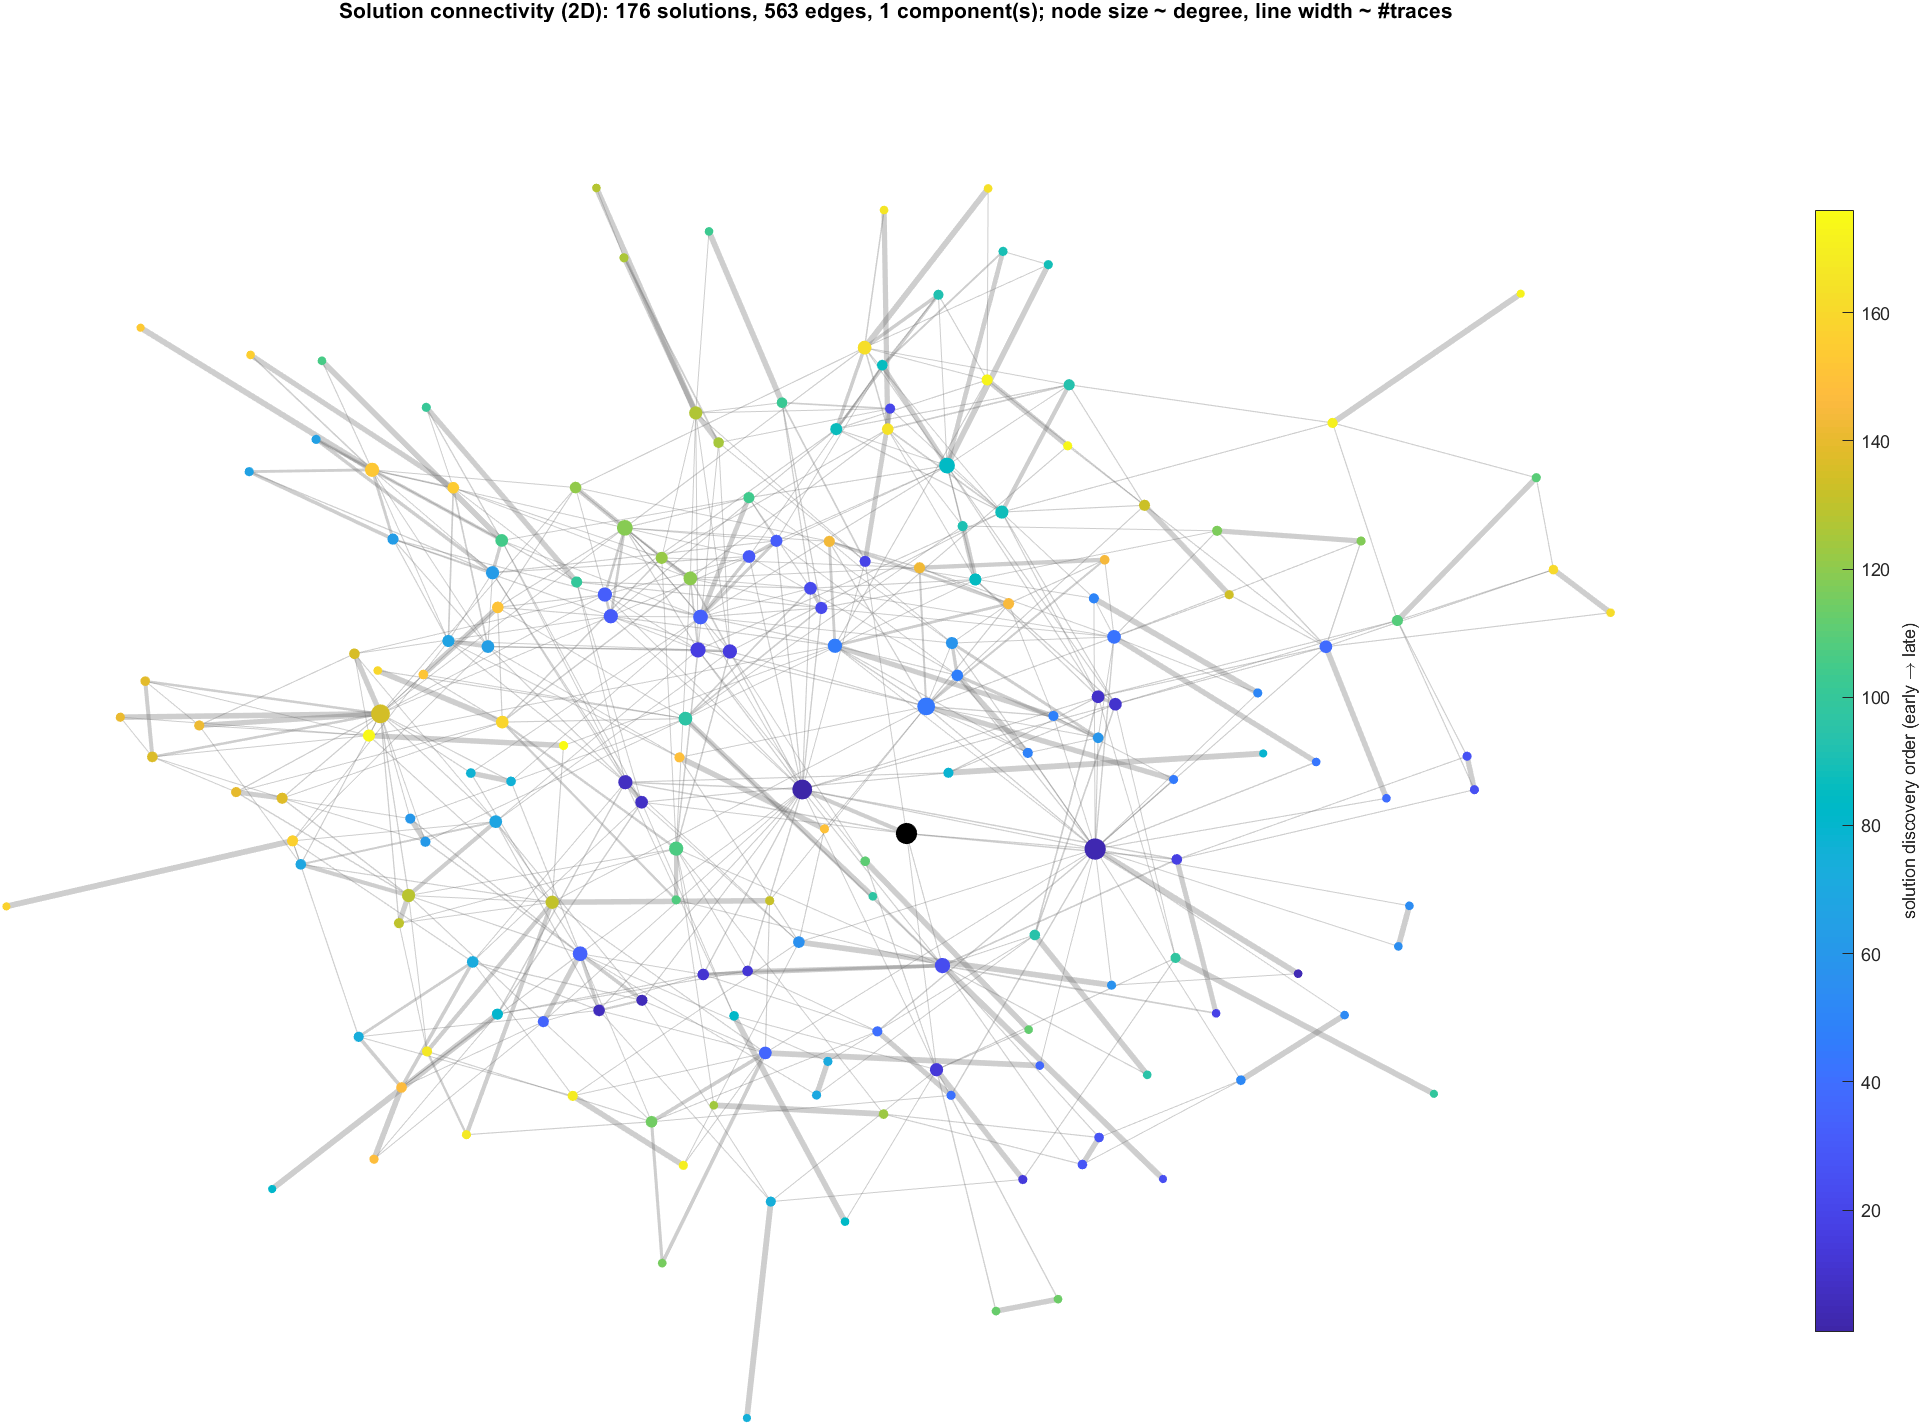
\includegraphics[width=0.30\textwidth]{connectivity_case39_bandit.png}&
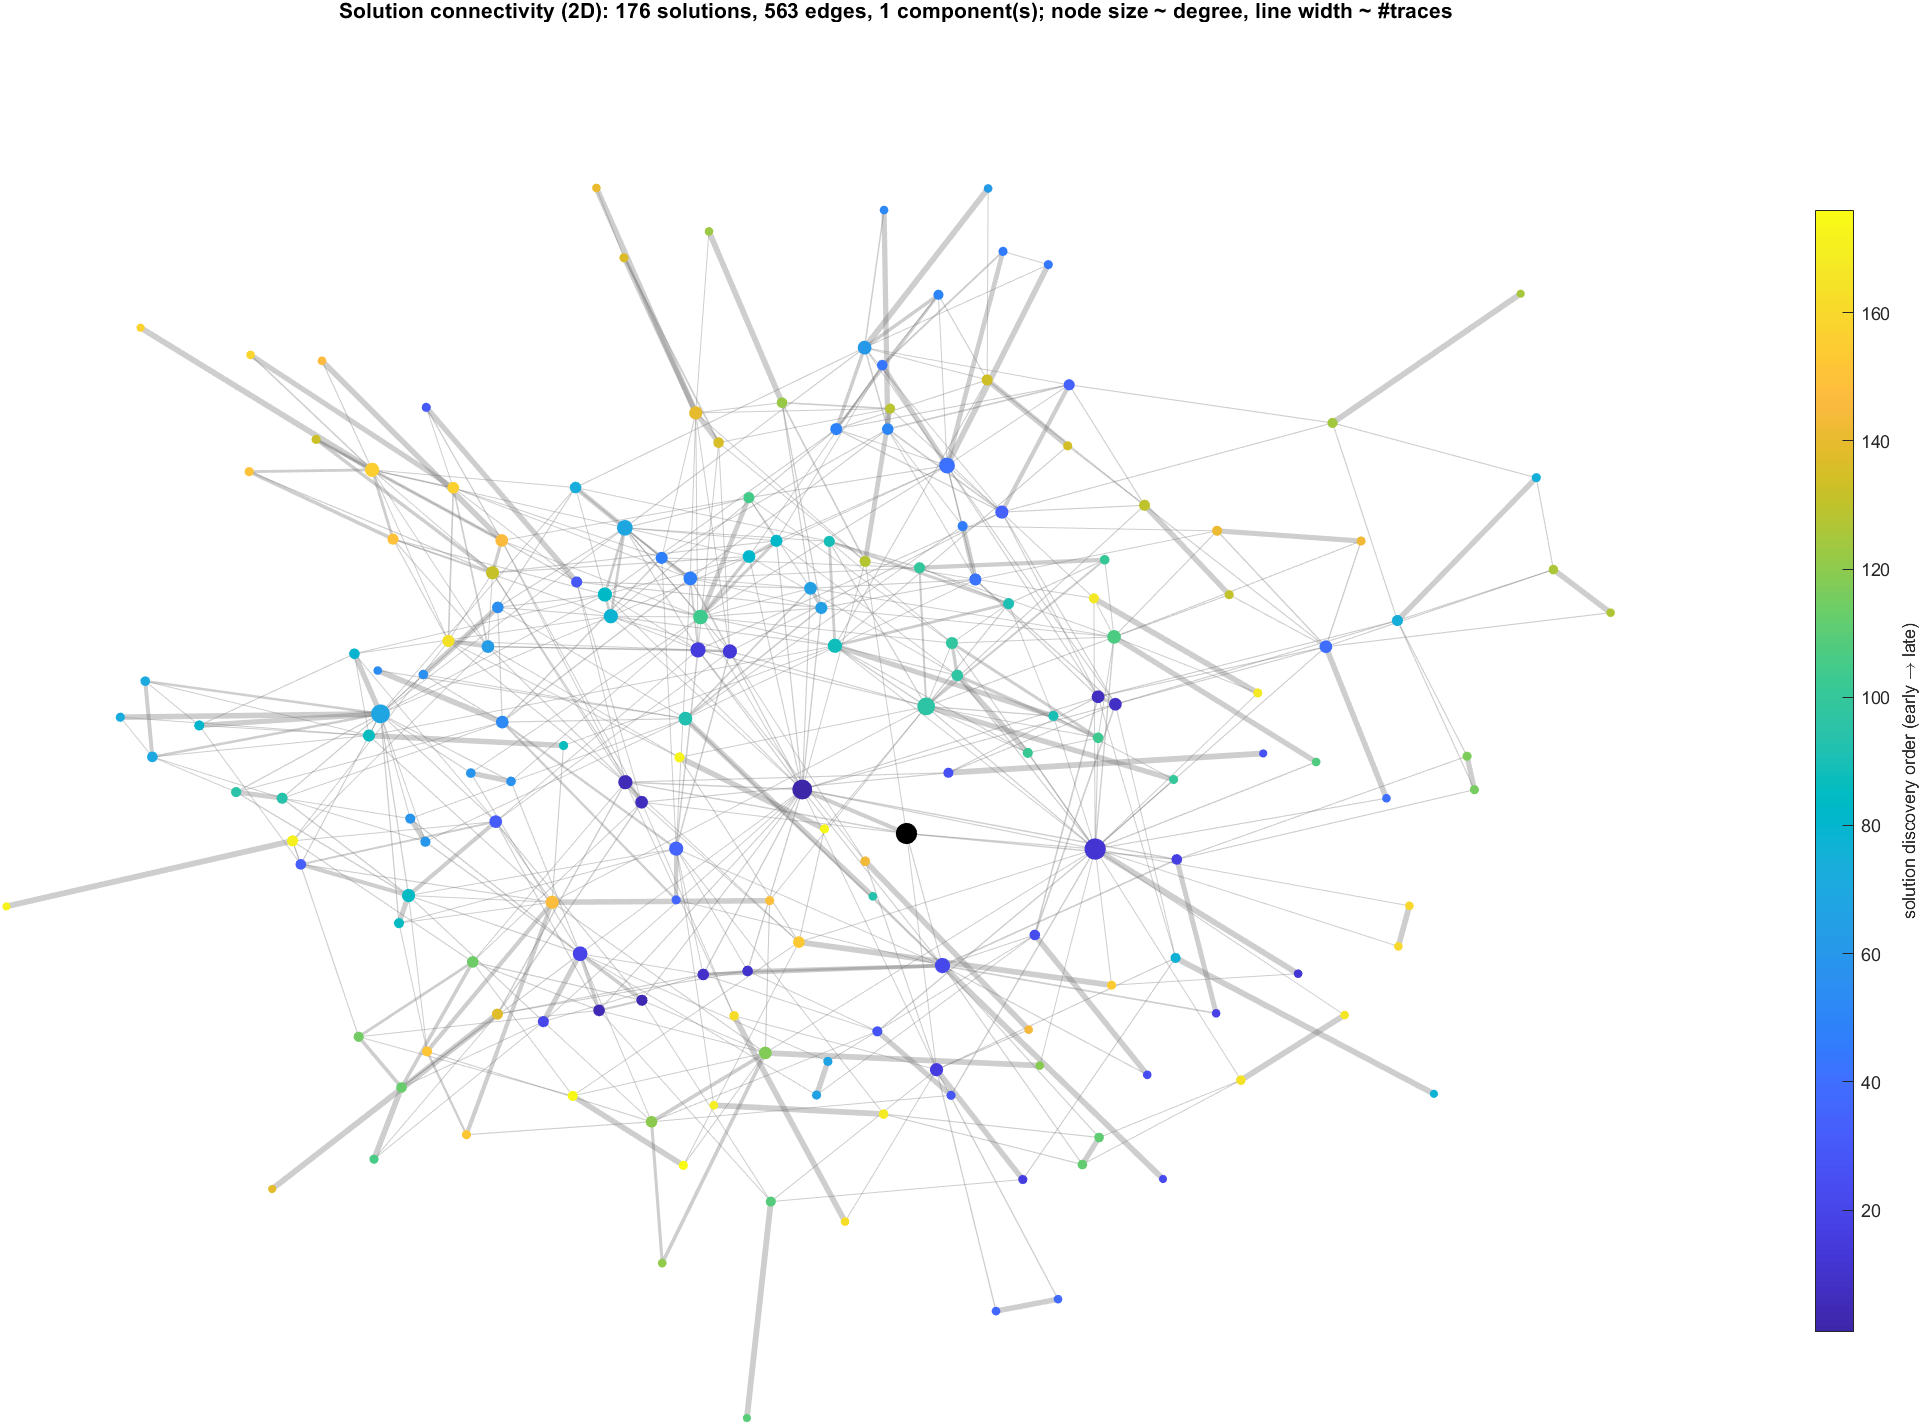
\includegraphics[width=0.30\textwidth]{connectivity_case39_novelty.png}\\
\code{scan}&\code{bandit}&\code{novelty}
\end{tabular}
\caption{case39 connectivity for the validated common 176-solution set.}
\end{figure}}{}

The scheduler benchmark retained final solution matrices and cumulative
per-trace discovery histories for case30 and case57, but it did not retain the
large policy-specific \code{VBook} arrays needed to reconstruct exact
scan/bandit/novelty edges. The following two figures are therefore explicitly
reference traversal graphs reconstructed offline from the complete released-v4
MEX snapshots. Their saved solution matrices agree with the v5 scan references
well inside the $4\times10^{-7}$ tolerance; they must not be interpreted as
three-policy v5 traversal comparisons.

\IfFileExists{connectivity_case30_v4_reference.png}{
\begin{figure}[p]\centering
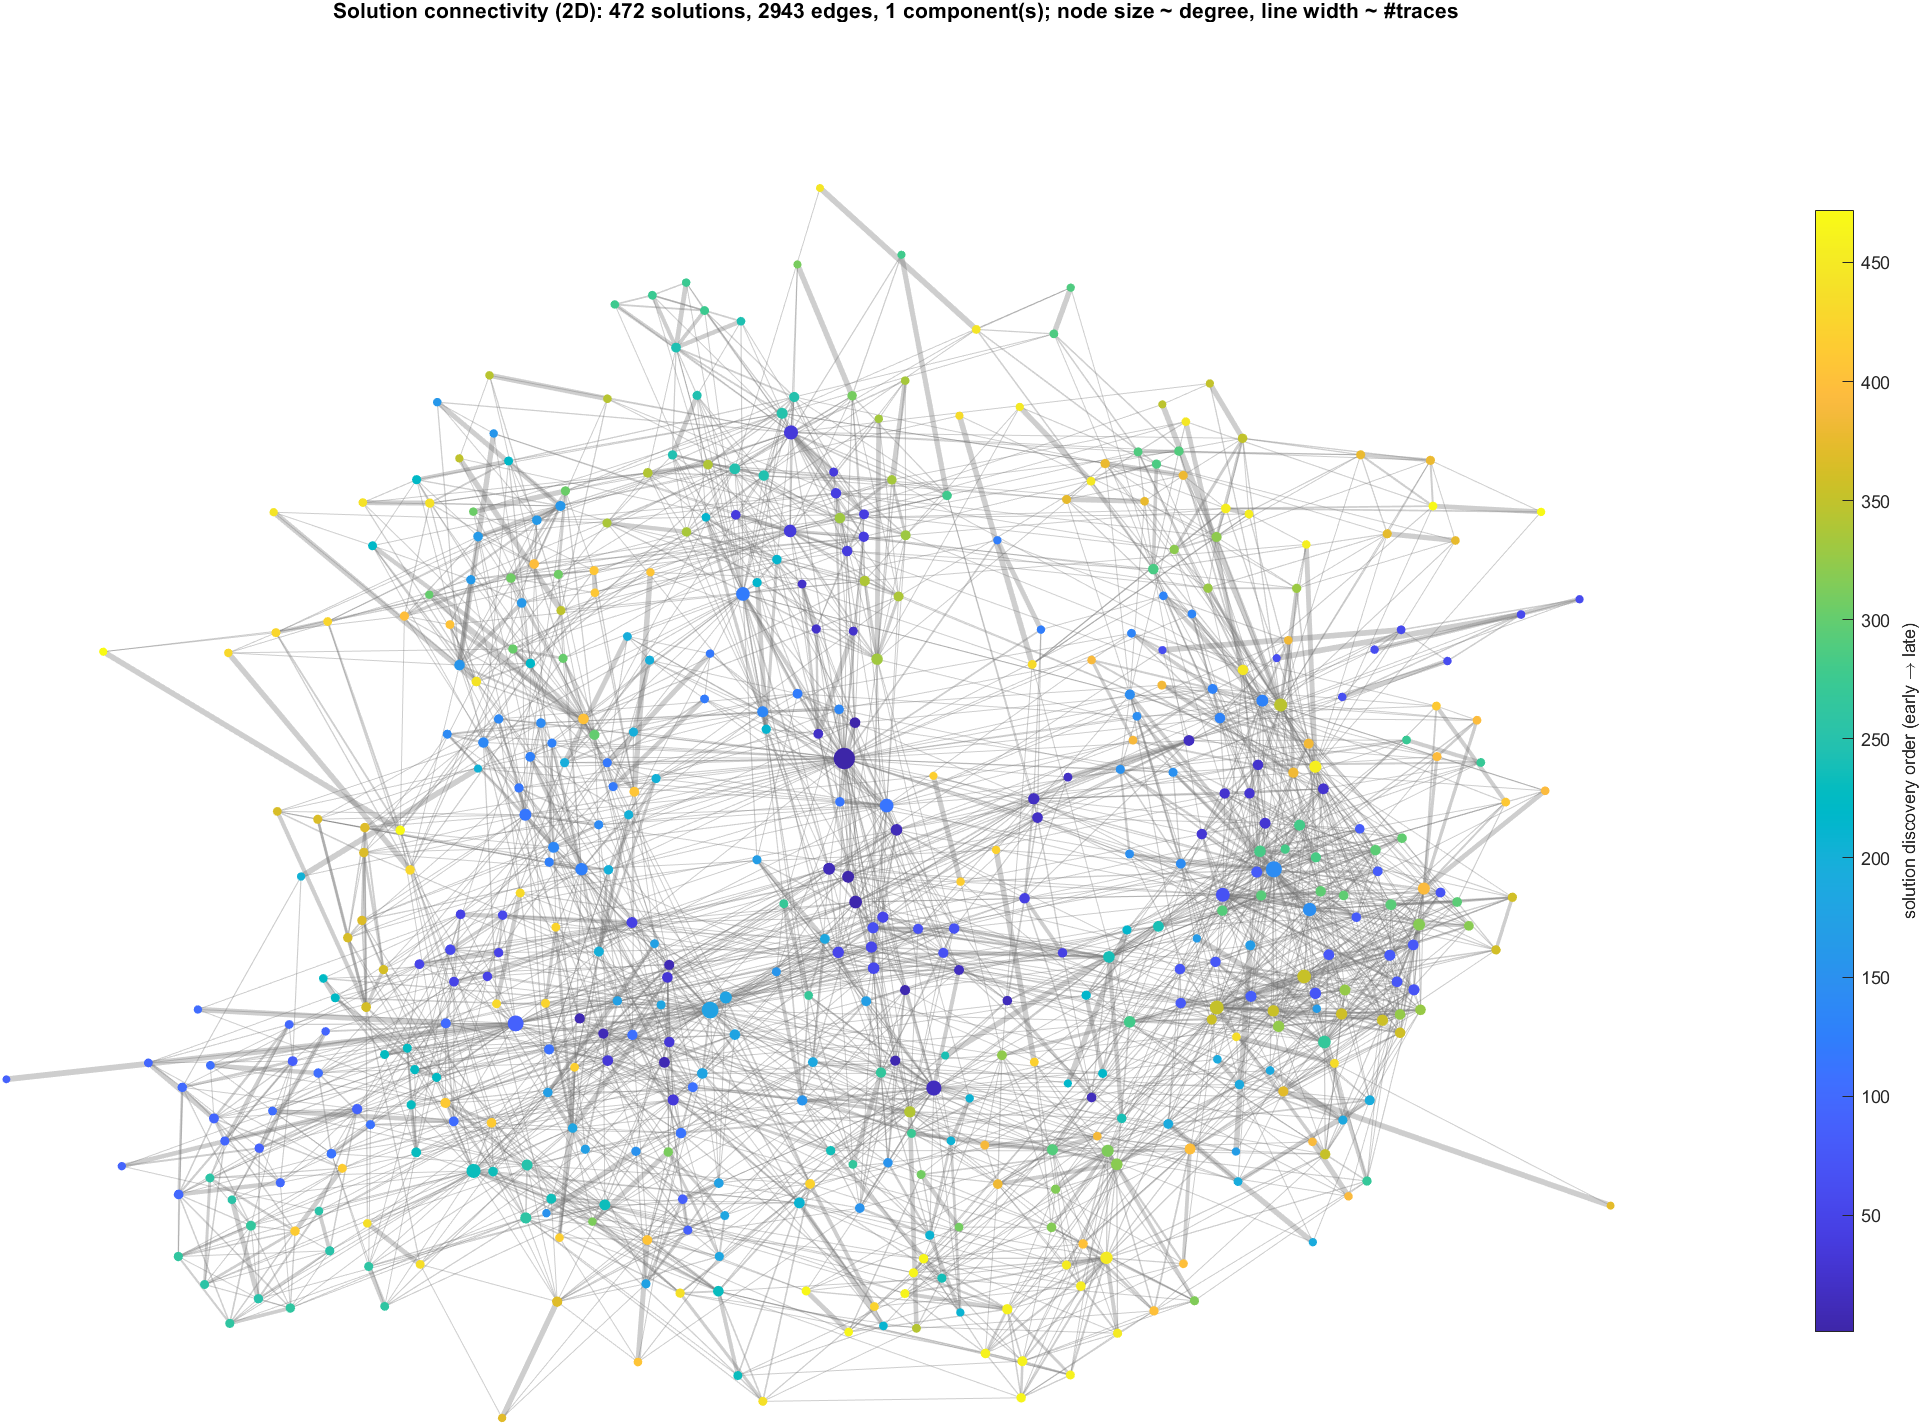
\includegraphics[width=0.96\textwidth]{connectivity_case30_v4_reference.png}
\caption{case30 released-v4 reference connectivity: 472 solutions, 2,943
unique edges, and one connected component. Node color records reference-run
discovery order; node size is degree and line width counts shared traces. The
solution-set distance to the saved v5 reference is $9.45\times10^{-12}$.}
\end{figure}}{}
\IfFileExists{connectivity_case57_v4_reference.png}{
\begin{figure}[p]\centering
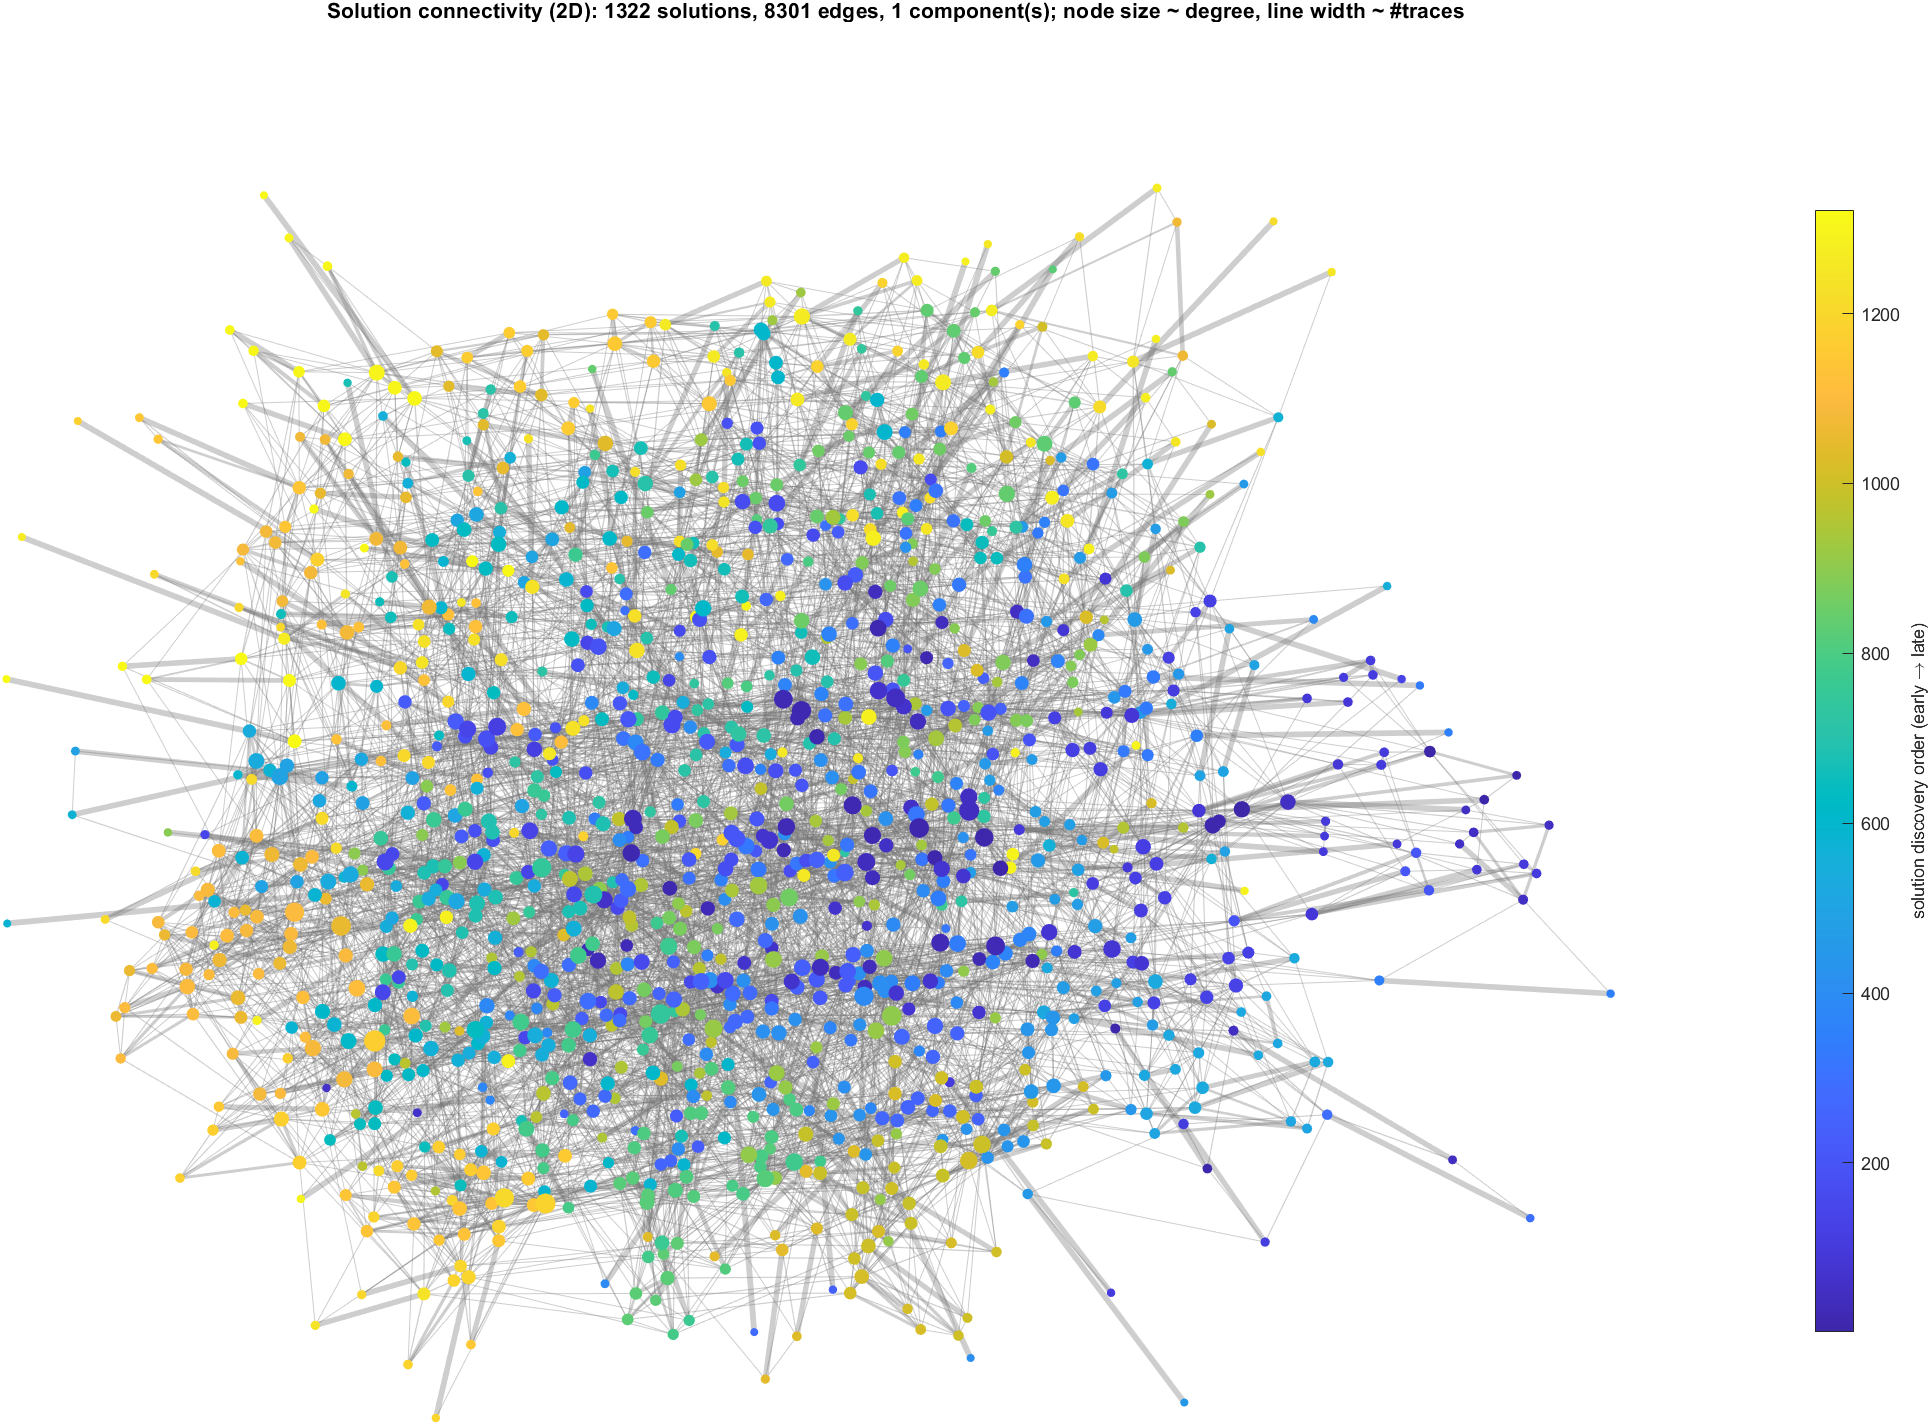
\includegraphics[width=0.96\textwidth]{connectivity_case57_v4_reference.png}
\caption{case57 released-v4 reference connectivity: 1,322 solutions, 8,301
unique edges, and one connected component. Node color records reference-run
discovery order; node size is degree and line width counts shared traces. The
solution-set distance to the saved v5 reference is $2.00\times10^{-10}$.}
\end{figure}}{}

All 180 timing runs returned expected counts. Independent symmetric nearest-set
validation passed 40/40 comparisons; worst distance was
$2.6591\times10^{-9}$ against a $4\times10^{-7}$ tolerance. The bundled
\code{test_checkpoint_policy_compatibility_v5.m} and \code{smoke_test_v5.m}
remain available for platform-specific checks, but results from non-designated
machines are not published. The full report and per-case table are in
\code{SCHEDULER_BENCHMARK_v5.md} and the published CSV files.

\section{Direct released-v4 performance baseline}
The retained v4 pass used the same 20 cases, MATLAB R2022a, Windows x64, and 23
workers. MEX v4 required 718.656~s and pure MATLAB v4 1272.966~s, both returning
3256 total solutions. V5 scan averaged 606.947~s, descriptively 15.5\% below
the historical MEX value. Because v4 is one retained pass and v5 is a current
three-repeat experiment, this is release context rather than a controlled paired
speedup claim.


\section{Choosing A Solver}

\begin{center}
\begin{tabular}{@{}p{0.28\textwidth}p{0.31\textwidth}p{0.31\textwidth}@{}}
\toprule
\textbf{Question} & \textbf{MEX v5} & \textbf{Pure MATLAB v5}\\
\midrule
Windows x64 MATLAB? & Recommended. Shipped \code{.mexw64} binaries are included. &
Works, but generally slower.\\
Linux or macOS? & Rebuild MEX binaries first, or use pure MATLAB. &
Recommended out of the box.\\
Need to inspect or modify hot-path code? & Possible, but rebuild if changing MEX source. &
Recommended for experimentation.\\
Need maximum speed? & Recommended. & Use when portability matters more than speed.\\
Need no compiler? & Works on Windows x64 with shipped binaries. &
Always works without a compiler.\\
\bottomrule
\end{tabular}
\end{center}

\section{Choosing A Mode}

Each solver has three main collection modes:

\begin{description}[leftmargin=0em,style=nextline]
\item[\code{serial}] Uses \code{runVBook_hybrid_2023.m}. It is the easiest mode to debug
and needs no Parallel Computing Toolbox.
\item[\code{parfor}] Uses \code{runVBook_hybrid_parallel.m}. It traces one row of
\code{VBook} at a time and waits for all equations in that row to finish.
\item[\code{parfeval}] Uses \code{runVBook_hybrid_parfeval.m}. It is asynchronous and keeps
workers busy without waiting for the slowest equation in each row. This is the recommended
mode for \code{case30}, \code{case39}, \code{case57mod}, \code{case57}, and larger systems.
\end{description}

The MEX folder also keeps \code{runVBook_hybrid_parfeval_barrier.m}. That file is a
retained comparison driver, not the recommended default.

\section{Recommended Configurations and Interpretation}

\begin{center}\small
\begin{tabular}{@{}p{0.28\textwidth}p{0.28\textwidth}p{0.34\textwidth}@{}}
\toprule
\textbf{Objective} & \textbf{Recommended configuration} & \textbf{Reason}\\
\midrule
Routine large-case enumeration & MEX + \code{parfeval} + \code{bandit} &
Best balance of early discovery, low selection overhead, and shipped acceleration.\\
Earliest broad solution sample & MEX + \code{parfeval} + \code{novelty} &
Strongest measured trace-to-90\% behavior, with extra scheduler work.\\
V4-oriented scheduler baseline & MEX + \code{parfeval} + \code{scan} &
Rotating first-eligible selection without learned or geometric ranking.\\
Portable or inspectable workflow & Pure MATLAB + \code{parfeval} + \code{bandit} &
No MEX dependency; use serial when the Parallel Computing Toolbox is unavailable.\\
\bottomrule
\end{tabular}
\end{center}

The following limits are important when interpreting the package and its measurements:

\begin{itemize}[leftmargin=1.4em]
  \item Scheduler policy changes queue order, not the HEBC equations or acceptance tests.
        Asynchronous completion can still change exact discovery order between runs.
  \item ``Total solutions'' in the benchmark is the solver's validated final output for
        that completed run. Trace-to-90\% uses 90\% of that run-final count; it is not an
        independent proof that every algebraic root exists in the returned set.
  \item The three-repeat comparison covers the 20 completed test cases through
        \code{case57}; \code{case118} is bundled as a test case but is excluded from the
        scheduler timing totals and completed-case validation claims.
  \item Wall times are machine- and worker-count-dependent. The v4 values are a retained
        historical baseline, whereas v5 uses three current repeats; their difference is
        descriptive release context rather than a controlled paired speedup.
  \item Run only one solver folder on the MATLAB path. MATPOWER is required; parallel
        modes additionally require the Parallel Computing Toolbox.
\end{itemize}

\section{Quick Start}

\begin{lstlisting}[style=mat]
cd('<path>/HEBCPF_MEX_v5')       % or HEBCPF_matlab_v5
addpath(pwd)

which runpf
which makeYbus

[result, solutions] = run_merged_case('case14mod', 'parfeval');
result
\end{lstlisting}

Batch entry points:

\begin{center}
\begin{tabular}{@{}ll@{}}
\toprule
\textbf{Driver} & \textbf{Mode}\\
\midrule
\code{run_batch.m} & serial\\
\code{run_batch_par.m} & \code{parfor}\\
\code{run_batch_parfeval.m} & queue \code{parfeval}\\
\bottomrule
\end{tabular}
\end{center}

\section{Resuming A Ceased Search}

The parallel v5 runbooks write periodic checkpoints to \code{temp_result.mat}. To resume:

\begin{enumerate}[leftmargin=1.6em]
  \item Return to the same solver folder.
  \item Use the same case, load factor, and driver mode.
  \item Load \code{temp_result.mat}.
  \item Run the matching runbook.
\end{enumerate}

\begin{lstlisting}[style=mat]
cd('<path>/HEBCPF_MEX_v5')       % or the pure MATLAB folder
addpath(pwd)
load temp_result.mat
wait = 0;
run('runVBook_hybrid_parfeval.m')         % queue parfeval checkpoint
% run('runVBook_hybrid_parallel.m')       % parfor checkpoint
\end{lstlisting}

For the MEX retained barrier driver:

\begin{lstlisting}[style=mat]
load temp_result.mat
wait = 0;
run('runVBook_hybrid_parfeval_barrier.m')
\end{lstlisting}

For serial runs, save the workspace manually before stopping:

\begin{lstlisting}[style=mat]
save('my_checkpoint.mat', '-v7.3')
load my_checkpoint.mat
wait = 0;
run('runVBook_hybrid_2023.m')
\end{lstlisting}

Internally, the resume path checks \code{VBook} and \code{Zsave}. If \code{Zsave} contains
extra preallocated columns, it is trimmed to the book-kept solution count. The queue
\code{parfeval} driver rebuilds per-equation cursors from \code{VBook == 0}; runtime futures and
parallel-pool objects are not restored from the checkpoint.

\section{Bundled Cases}

\begin{center}\small
\begin{tabular}{@{}p{0.19\linewidth}p{0.27\linewidth}p{0.18\linewidth}p{0.28\linewidth}@{}}
\toprule
\code{case3} (6) & \code{case4gs} (6) & \code{case4BB0} (14) & \code{case4BBc} (12)\\
\code{case5loop} (10) & \code{case5Salam} (10) & \code{case6ww} (6) & \code{case7Salam} (4)\\
\code{case9} (8) & \code{case9Q} (8) & \code{case14mod} (30) & \code{case33bw} (16)\\
\code{case39} (176) & \code{case30}/\code{case_ieee30} (472) & \code{case57mod} (606) & \code{case57} (1322)\\
\multicolumn{4}{c}{\code{case118}: bundled test case; no completed reference count claimed}\\
\bottomrule
\end{tabular}
\end{center}

Counts above are nominal-load reference counts for the completed bundled benchmarks,
collapsing antipodal duplicates in the solver's canonical output convention.

\section{Official Validation Summary}

The official code{20260724_3x23} dataset records scheduler timing and
order-independent solution-set validation on the designated main job machine:

\begin{center}
\small
\setlength{\tabcolsep}{3pt}
\begin{tabular}{@{}>{\raggedright\arraybackslash}p{0.17\linewidth}
>{\raggedright\arraybackslash}p{0.24\linewidth}
>{\raggedright\arraybackslash}p{0.16\linewidth}
>{\raggedright\arraybackslash}p{0.27\linewidth}@{}}
\toprule
\textbf{Folder} & \textbf{Driver} & \textbf{Cases} & \textbf{Result}\\
\midrule
MEX v5 & three schedulers, three repeats & all 20 cases through case57 &
180/180 timing runs returned expected counts.\\
MEX v5 & order-independent solution audit & all 20 cases &
40/40 checks passed; worst distance $2.6591\times10^{-9}$.\\
\bottomrule
\end{tabular}
\end{center}

The user guides were checked against the actual runbooks for checkpoint name,
resume path, driver names, and \code{slope_max = 4e5}. Checkpoint and smoke-test
harnesses are included for platform-specific verification, but results from
non-designated machines are not presented as release evidence.

\section{Release Contents}

\begin{center}\small
\begin{longtable}{@{}p{0.30\textwidth}p{0.60\textwidth}@{}}
\toprule
\textbf{Path} & \textbf{Purpose}\\
\midrule\endhead
\code{README.md} & GitHub front page and quick start.\\
\code{CHANGELOG.md} & Release history.\\
\code{RELEASE_NOTES_V5.md} & GitHub release notes for this package.\\
\code{RELEASE_CHECKLIST_V5.md} & Pre-upload package and release-asset checklist.\\
\code{CITATION.cff} & Software citation metadata.\\
\code{LICENSE}, \code{NOTICE} & License and third-party notices.\\
\code{HEBCPF_Suite_Overview.tex/pdf} & This overview.\\
\code{HEBCPF_MEX_v5/} & Compiled Windows x64 v5 solver.\\
\code{HEBCPF_matlab_v5/} & Pure MATLAB v5 solver.\\
\code{SCHEDULER_BENCHMARK_v5.md} & Full three-policy benchmark report and interpretation.\\
\code{BENCHMARK_METADATA_v5.json} & Official dataset identity, platform,
scheduler parameters, and provenance.\\
GitHub Release benchmark asset & Portable benchmark CSV files, validation data,
trace histories, references, and SHA-256 checksum; attached separately rather
than committed to Git.\\
GitHub Release KLU assets & V5 MEX binary, exact pinned corresponding source,
license texts, build metadata, and SHA-256 checksums.\\
\code{klurf/} & KLU refactor MEX wrapper, build helper, binary, and notes.\\
\bottomrule
\end{longtable}
\end{center}

\section{Citation}

If you use results produced by this solver, please cite:

\begin{quote}
D. Wu and B. Wang, ``Holomorphic Embedding Based Continuation Method for Identifying
Multiple Power Flow Solutions,'' \emph{IEEE Access}, vol. 7, pp. 86843--86853, 2019.
doi: \href{https://doi.org/10.1109/ACCESS.2019.2925384}{10.1109/ACCESS.2019.2925384}.
\end{quote}

For citing the software package, use the included \code{CITATION.cff}.

\end{document}
